\documentclass[germanthesis]{thesis-style}
% options:
% [germanthesis] - Thesis is written in German
% [plainunnumbered] - Don't print numbers on plain pages
% [earlydraft] - Settings for quick draft printouts
% [watermark] - Print current time/date at bottom of each page
% [phdthesis] - switch to PhD thesis style
% [twoside] - double sided
% [cutmargins] - text body fills complete page

% Extension to BibLaTex (useful for cites in footnotes)
%\usepackage[backend=bibtex, style=numeric-comp]{biblatex}
\bibliography{references}

\author{Martin~Nocker}
\title{R-Paket für Kanalkodierung mit Faltungskodes}
%\title{R~package for channel~coding with convolutional~codes}
\birthday{1. Mai 1993}
\birthplace{Innsbruck}
%\thesisstart{20. Oktober 2015}
\thesistype{Bachelor's thesis}
\thesistypegerman{Bachelorarbeit}
\thesiscite{Bachelor's thesis}
\advisors{Univ.-Prof.~Dr.~Rainer~Böhme, Dr.~Pascal~Schöttle}

% additional packages
\usepackage{color, colortbl} % colors (interface table)
\usepackage{longtable}
\usepackage{amsmath}
\usepackage{graphicx}
\usepackage{caption}
\usepackage{subcaption}
\usepackage{tikz}
\usetikzlibrary{backgrounds, calc, positioning}
% für \FloatBarrier Befehl
\usepackage{placeins}

% Caption von longtables ändern (Tabelle -> Funktion)
\captionsetup[longtable]{name=Funktion}

% zentrieren der subcaptions
\captionsetup[subfigure]{justification=centering}

% Listings standardmaessig in R
\lstset{language=R, basicstyle=\ttfamily\footnotesize, prebreak={}}

% Theorems
\usepackage{amsthm}
\newtheorem{mytheorem}{Theorem}
\newtheorem{beispiel}{Beispiel}

% Definiert Makro für Grafik Skalierung
\makeatletter
\def\ScaleIfNeeded{%
\ifdim\Gin@nat@width>\linewidth
\linewidth
\else
\Gin@nat@width
\fi
}
\makeatother

\newcommand{\plotwidth}{0.6\textwidth}
\begin{document}

% Titelseiten und Eidesstattliche Erklärung
\maketitle

% Zusammenfassung
\begin{abstract}
Diese Bachelorarbeit implementiert das Turbo-Kode-Verfahren, verpackt in einem R-Paket. Diese Kodierung ist ein Teilgebiet der Kanalkodierung, die bei heutigen Kommunikationskanälen nicht mehr wegzudenken ist, da auftretende Fehler während der Übertragung der Nachricht, dadurch wieder rekonstruierbar sind. Hauptanwendungsgebiet sind dabei die Mobil- und Satellitenkommunikation, da hierbei wichtig ist, dass eine Nachricht nicht mehrmals übertragen werden muss, bis sie korrekt ankommt. Um für zukünftige Studierende das Erlernen dieser Kommunikationstechnik zu erleichtern, sollten geeignete Visualisierungen geschaffen werden. Diese Arbeit steht in enger Verbindung mit den beiden Bachelorarbeiten, die Blockkodierung und Faltungskodierung behandeln. Alle drei Kodierungsverfahren sollten in das selbe R-Paket inkludiert werden.

\end{abstract}

\tableofcontents
\clearpage
\pagenumbering{arabic}

\chapter{Einleitung}
\label{kapitel:einleitung}
% einleitung.tex
\section{Motivation}
Lorem Ipsum
\\
\\
\section{Ziel}

\chapter{Grundlagen}
\label{kapitel:grundlagen}
% grundlagen.tex
In Kapitel~\ref{kapitel:grundlagen_kanalkodierung} werden Prinzipien und Eigenschaften der Kanalkodierung beschrieben. Kapitel~\ref{kapitel:grundlagen_faltungskodierung} geht auf Faltungskodes ein, eine Art der Kanalkodierung auf die sich diese Arbeit konzentriert. Der Inhalt dieser Kapitel orientiert sich an \cite{huffman2010fundamentals}, sowie \cite{morelos2006art} und~\cite{schonfeld2012informations}.
\section{Kanalkodierung}
\label{kapitel:grundlagen_kanalkodierung}
\begin{figure}[t]
\centering
\resizebox{\textwidth}{!}{%
	% kommunikationskanal.tex
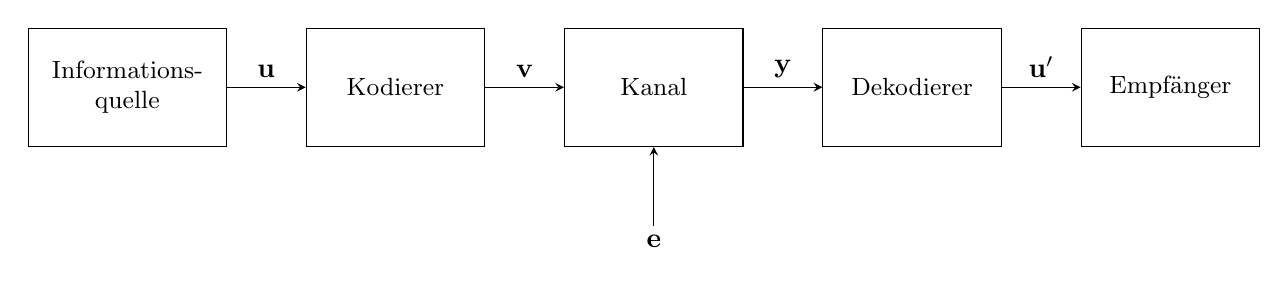
\begin{tikzpicture}[>=stealth]
\def\myinnersep{3mm}
\tikzstyle{block} = [draw, rectangle, node distance=10mm, inner sep=\myinnersep, align=center, font=\small, minimum height=15mm, minimum width=width("Dekodierer")+2*\myinnersep]
\node[block] (quelle) {Informations- \\ quelle};
\node[block] (kodierer) [right=of quelle] {Kodierer};
\node[block] (kanal) [right=of kodierer] {Kanal};
\node[block] (dekodierer) [right=of kanal] {Dekodierer};
\node[block] (senke) [right=of dekodierer] {Empfänger};
\draw[->] (quelle) -- node [above] {$\mathbf{u}$} (kodierer);
\draw[->] (kodierer) -- node [above] {$\mathbf{v}$} (kanal);
\draw[->] (kanal) -- node [above] {$\mathbf{y}$} (dekodierer);
\draw[->] (dekodierer) -- node [above] {$\mathbf{u'}$} (senke);
\draw[<-] (kanal.south) -- ++(0,-10mm) node [below] {$\mathbf{e}$};
\end{tikzpicture}
}
\caption{Kommunikationskanal}
\label{abb:kommunikationskanal}
\end{figure}
Kanalkodierung kann als Zuordnung bzw. Abbildung von Quellzeichen zu Kanalzeichen angesehen werden. Quellzeichen sind Zeichen, die eine Informationsquelle emittiert. Kanalzeichen sind Zeichen, die über einen Kommunikationskanal übertragen werden. Der Kanal enthält ein Rauschen, d.h. Informationen die von der Quelle emittiert werden, können verändert beim Empfänger ankommen. Daher wird der Kanal als \emph{verrauschter} Kanal bezeichnet. Würde eine Information unkodiert über den verrauschten Kanal übertragen werden, könnte die verfälschte Nachricht nicht wiederhergestellt werden. Daher fügt ein Kanalkodierer den Quellzeichen Redundanz hinzu, sodass empfängerseitig verfälschte Zeichen erkannt und korrigiert werden können.

Abbildung~\ref{abb:kommunikationskanal} zeigt einen Kommunikationskanal. Eine Nachricht $\mathbf{u}=\left( u_{1},u_{2},\dots ,u_{k}\right)$ wird in ein Kodewort $\mathbf{v}=\left( v_{1},v_{2},\dots ,v_{n}\right)$, welches Redundanz enthält, kodiert. Vor der Übertragung über den Kanal werden die Bits folgendermaßen auf die Signalpegel +1 bzw. -1 abgebildet:
\begin{equation}
\text{Signal(Bit)} =
\begin{cases}
  +1  & \quad \text{wenn Bit} = 0\\
  -1  & \quad \text{wenn Bit} = 1\\
\end{cases}
\label{eq:bit_zu_signal_abbildung}
\end{equation}
Bei der Übertragung wird das Signal durch Rauschen, welches als Fehlervektor $\mathbf{e}=\left( e_{1},e_{2},\dots ,e_{n}\right)$ dargestellt wird, verfälscht. Der Empfangsvektor $\mathbf{y}$ ergibt sich aus der Überlagerung von $\mathbf{v}$ und $\mathbf{e}$. Der Empfangsvektor wird vor der Dekodierung von den Signalpegeln zurück auf die Bit-Werte 0 bzw. 1 abgebildet.
\begin{equation}
\text{Kode(Signal)} =
\begin{cases}
  0  & \quad \text{wenn Signal } \geq 0\\
  1  & \quad \text{sonst}\\
\end{cases}
\label{eq:signal_zu_bit_abbildung}
\end{equation}
Das daraus resultierende Kodewort wird vom Dekodierer zur Schätzung $\mathbf{u'}$ der originalen Nachricht dekodiert. Ziel der Kanalkodierung ist, dass die Wahrscheinlichkeit von $\mathbf{u'}=\mathbf{u}$ maximiert wird.

\subsection{Koderate}
\label{kapitel:grundlagen_koderate}
Die Koderate $R$ eines Kodes beschreibt das Verhältnis der Länge zwischen dem Quellwort $\mathbf{u}=\left( u_{1},u_{2},\dots ,u_{k}\right)$ und dem Kodewort $\mathbf{v}=\left( v_{1},v_{2},\dots ,v_{n}\right)$.
\begin{equation}
R=\frac{k}{n}<1
\end{equation}
Wobei $k$ bzw. $n$ den Längen des Quellworts bzw. Kodeworts entsprechen. Somit beschreibt die Koderate das Verhältnis zwischen Information und Redundanz im übertragenen Kodewort. Bei hoher Redundanz ergibt sich eine niedrige Koderate. Die Übertragung ein und derselben Information bei gleicher Übertragungsgeschwindigkeit dauert bei Kodes mit niedriger Koderate länger, als bei Kodes mit höherer Koderate.
\pagebreak
\subsection{Hamming-Distanz}
\label{kapitel:grundlagen_hamming_distanz}
Die Hamming-Distanz $d$ (auch $d_{H}$) zweier Kodewörter $\mathbf{a}=\left( a_{1},a_{2},\dots ,a_{n}\right)$ und $\mathbf{b}=\left( b_{1},b_{2},\dots ,b_{n}\right)$ entspricht der Anzahl an Stellen, in denen sich die beiden Kodewörter unterscheiden:
\begin{equation}
d(a,b)=\vert\left\lbrace i \in \left\lbrace 1,2,\dots ,n \right\rbrace\vert a_{i}\neq b_{i}\right\rbrace\vert\; .
\end{equation}
Für binäre Kodewörter ergibt sich die Hamming-Distanz aus der binären Addition der Kodewörter:
\begin{equation}
d(a,b)=\sum_{i=1}^{n} \left( a_{i} \oplus b_{i}\right).
\end{equation}
Das Hamming-Gewicht $w$ eines binären Kodeworts $\mathbf{a}=\left( a_{1},a_{2},\dots ,a_{n}\right)$ entspricht der Anzahl an Bits im Wort, für die gilt $a_{i}=1$ mit $i \in \left\lbrace 1,2,\dots ,n \right\rbrace$.
\begin{equation}
w(a)=\vert\left\lbrace i \in \left\lbrace 1,2,\dots ,n \right\rbrace\vert a_{i}=1\right\rbrace\vert=\sum_{i=1}^{n} a_{i}
\end{equation}

\section{Faltungskodierung}
\label{kapitel:grundlagen_faltungskodierung}
Faltungskodes sind blockfreie Kodes, d.h. Quellzeichen werden nicht in Blöcke fester Länge unterteilt, vielmehr wird ein Informationsstrom kodiert, sodass ein einziges Kodewort resultiert. Ein weiterer Unterschied zu Blockkodes besteht darin, dass Kodebits nicht nur vom aktuellen Eingangsbit abhängen, sondern auch von vorherigen Eingangsbits. Die Redundanz wird bei Faltungskodes kontinuierlich in das Kodewort eingefügt. Im Allgemeinen können Faltungskodierer beliebig viele Eingänge haben, sodass mehrere Informationsbits gleichzeitig kodiert werden. Trotz besserer Koderate bei Kodierern mit mehreren Eingängen sind nur Kodierer mit einem Eingang von praktischer Relevanz. Im Folgenden werden nur noch Faltungskodierer mit einem Eingang betrachtet.

\subsection{Kodiererdarstellung und Kodierung}
\label{kapitel:grundlagen_darstellung}
Faltungskodierer lassen sich einfach durch ein Schieberegister und mehrere logische XOR-Gatter darstellen. Bei einem Faltungskodierer mit $N$ Ausgängen und einem Schieberegister der Länge $M$ wird ein Eingangsbit $u \in \left\lbrace 0,1 \right\rbrace$ in eine Kodesequenz $\mathbf{v}$ der Länge $N$ $\left( \mathbf{v} \in {\left\lbrace 0,1\right\rbrace }^{N}\right)$ kodiert. Es ergibt sich somit eine Koderate von $R=\frac{1}{N}$. Ein Ausgang wird durch ein sogenanntes \emph{Generatorpolynom} definiert. Ein Generatorpolynom stellt eine Linearkombination der $M$ Elemente des Schieberegisters und dem Eingangssignal dar und wird durch ein XOR-Gatter abgebildet. Alle Generatorpolynome werden in einer \emph{Generatormatrix}
\begin{equation}
G=\left( g_{1}, g_{2},\dots , g_{N} \right) 
\end{equation}
angegeben, wobei das Generatorpolynom $g_{i}$ den Ausgang $i$ definiert. Zur Definition eines Faltungskodierers im praktischen Teil der Arbeit müssen die Generatorpolynome angegeben werden.
\\
Ein weiterer wichtiger Parameter von Faltungskodes ist die \emph{Einflusslänge} (constraint length). Diese gibt an, wie oft sich ein Eingangsbit auf die Kodierung auswirkt. Die Einflusslänge wird durch die Länge des Schieberegisters bestimmt. Ein Eingangsbit beeinflusst $M+1$ mal die Kodierung.
\\
\\
Die Verhaltensweise eines Faltungskodierers kann durch seinen \emph{Zustandsgraphen} beschrieben werden. Ein Zustand entspricht einer bestimmten Bitbelegung des Schieberegisters. Für einen Faltungskodierer mit einem Schieberegister der Länge $M$ ergeben sich $2^{M}$ Zustände. Faltungskodierer starten, falls nicht explizit angegeben, im Nullzustand, d.h. die Elemente des Schieberegisters sind mit 0 initialisiert.
\begin{figure}[t]
	\centering
	\begin{subfigure}{0.65\textwidth}
		\centering
		\resizebox{0.99\textwidth}{!}{%
			% standardkodierer.tex
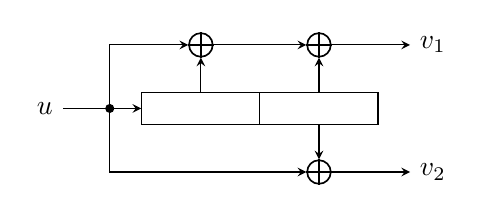
\begin{tikzpicture}[>=stealth]
\tikzstyle{rect} = [draw, rectangle, minimum width=30mm, inner sep=0mm, minimum height=4mm]
\tikzstyle{xor} = [draw, circle, semithick, minimum size=3mm, inner sep=0mm]

\node[rect] (rect) {};
\draw[-] (rect.north) -- (rect.south);
\draw[<-] (rect.west) -- ++(-10mm,0) node [left] {$u$};

\node[xor] (xor1) at ($(rect.north)+(-7.5mm,6mm)$) {};
\draw[semithick] (xor1.north) -- (xor1.south);
\draw[semithick] (xor1.west) -- (xor1.east);
\draw[->] ($(rect.north)+(-7.5mm,0)$) -- (xor1.south);

\node[xor] (xor2) at ($(rect.north)+(7.5mm,6mm)$) {};
\draw[semithick] (xor2.north) -- (xor2.south);
\draw[semithick] (xor2.west) -- (xor2.east);
\draw[->] ($(rect.north)+(7.5mm,0)$) -- (xor2.south);

\node[xor] (xor3) at ($(rect.south)+(7.5mm,-6mm)$) {};
\draw[semithick] (xor3.north) -- (xor3.south);
\draw[semithick] (xor3.west) -- (xor3.east);
\draw[->] ($(rect.south)+(7.5mm,0)$) -- (xor3.north);

\draw[->] ($(rect.west)+(-4mm,0)$) |- (xor1.west);
\draw[->] (xor1.east) -- (xor2.west);
\draw[->] (xor2.east) -- ($(rect.north east)+(4mm,6mm)$) node [right] {$v_{1}$};

\draw[->] ($(rect.west)+(-4mm,0)$) |- (xor3.west);
\draw[->] (xor3.east) -- ($(rect.south east)+(4mm,-6mm)$) node [right] {$v_{2}$};

\draw[black, fill=black] ($(rect.west)+(-4mm,0)$) circle [radius=.5mm];
\end{tikzpicture}
		}
		\caption{Schaltbild}
		\label{abb:bsp1_schaltbild}
	\end{subfigure}
	~ % spacing between subfigures
	\begin{subfigure}{0.3\textwidth}
		\centering
		\resizebox{0.99\textwidth}{!}{%
			% zustandsdiagramm.tex
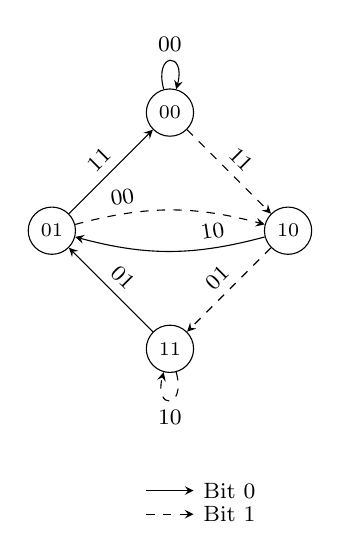
\begin{tikzpicture}[>=stealth, font=\footnotesize, scale=.6]
\tikzstyle{state} = [draw, circle, inner sep=1mm, minimum size=6mm, font=\scriptsize]
\node[state] (state0) at ( 0.0, 2.5) {$00$};
\node[state] (state2) at ( 2.5, 0.0) {$10$};
\node[state] (state3) at ( 0.0,-2.5) {$11$};
\node[state] (state1) at (-2.5, 0.0) {$01$};
\draw[->] (state0) to [looseness=8,out=105,in=75] node [sloped, above] {$00$} (state0);
\draw[->, dashed] (state0) to  node [sloped, above] {$11$} (state2);
\draw[->] (state1) to  node [sloped, above] {$11$} (state0);
\draw[->, dashed] (state1) to [bend left=15] node [sloped, above,near start] {$00$} (state2);
\draw[->] (state2) to [bend left=15] node [sloped, above,near start] {$10$} (state1);
\draw[->, dashed] (state2) to  node [sloped, above] {$01$} (state3);
\draw[->] (state3) to  node [sloped, above] {$01$} (state1);
\draw[->, dashed] (state3) to [looseness=8,out=285,in=255] node [sloped, below] {$10$} (state3);
\draw [->] ($(state3)+(-.5,-3)$) node (bit0) {} -- ++(1,0) node [right] {Bit 0};
\draw [->, dashed] ($(bit0)+(0,-.5)$) -- ++(1,0) node [right] {Bit 1};
\end{tikzpicture}
		}
		\caption{Zustandsdiagramm}
		\label{abb:bsp1_zustandsdiagramm}
	\end{subfigure}
	\caption{Beispiel für Faltungskodierer}
	\label{abb:standardkodierer}
\end{figure}
\begin{beispiel} Ein Faltungskodierer ist gegeben durch das Schaltbild bzw. Zustandsdiagramm in Abbildung~\ref{abb:standardkodierer}. Der Faltungskodierer besitzt die Generatormatrix 
\begin{equation*}
G=\left(7_{8},5_{8}\right) = \begin{pmatrix}
111 \\
101 \\
\end{pmatrix} = \left(1+D+D^{2}, 1+D^{2} \right)
\end{equation*}
\label{bsp:B1}
\end{beispiel}
Beispiel~\ref{bsp:B1} zeigt die verschiedenen Notationen für die Generatormatrix. Die am häufigsten verwendete Schreibweise ist die Darstellung der Generatorpolynome in oktaler Form. Dabei werden die Polynome in binärer Schreibweise konzise zu oktalen Zahlen zusammengefasst. Bei der binären Schreibweise entspricht die Bitposition des Polynoms dem Element im Schaltbild, d.h. das Most Significant Bit (MSB) des Polynoms steht für das Eingangssignal, das Least Significant Bit (LSB) des Polynoms steht für den Inhalt des letzten (am weitesten rechts liegenden) Elements des Schieberegisters. In die Linearkombination zur Definition des Ausgangssignals werden jene Elemente miteinbezogen, an deren Stelle im binären Polynom eine 1 steht. In \cite{huffman2010fundamentals} wird die Notation der binären Polynome über der Variable $D$ (\enquote{delay}) eingeführt. Das Eingangssignal und die Schieberegisterelemente entsprechen einer Potenz von $D$, wobei das Eingangssignal $u$ der Potenz $D^{0}=1$ und das letzte Schieberegisterelement $D^{M}$ entspricht. Das Generatorpolynom ergibt sich aus der Summe aller Potenzen deren Elemente Teil der Linearkombination sind. Darüber hinaus wird in Abbildung~\ref{abb:bsp1_zustandsdiagramm} das Zustandsdiagramm abgebildet. Die Knoten stellen die Zustände des Kodierer, d.h. die Belegungen des Schieberegisters, dar. Die gerichteten Kanten entsprechen einem Übergang bei einem Eingangsbit, wobei eine durchgezogene Kante einer 0 als Eingangsbit entspricht und eine gestrichelte Kante einer 1. Die Kantenbewertungen entsprechen den Ausgangsbits.

\begin{beispiel} Gegeben sei der Faltungskodierer aus Beispiel~\ref{bsp:B1}. Eine Nachricht $\mathbf{u}=\left( 110100\right)$ wird in den Kode $\mathbf{v}=\left( 11~01~01~00~10~11\right)$ kodiert.
\label{bsp:B2}
\end{beispiel}

\subsection{Dekodierung}
\label{kapitel:grundlagen_dekodierung}
\begin{figure}[t]
	\centering
	%\resizebox{\textwidth}{!}
\caption{Trellis für die Kodierung zu Beispiel~\ref{bsp:B2}}
\label{abb:trellis_kodierung}
\end{figure}
Zur Dekodierung von Faltungskodes wird der \emph{Viterbi-Algorithmus} angewendet. Der Algorithmus verwendet zur Dekodierung einer Kodesequenz das \emph{Trellis-Diagramm} (kurz: Trellis). Abbildung~\ref{abb:trellis_kodierung} zeigt das Trellis zur Kodierung der Nachricht aus Beispiel~\ref{bsp:B2}. Das Trellis ist eine Erweiterung des Zustandsdiagramms um eine Zeitachse auf der Abszisse. Die Zustände sind auf der Ordinate aufgetragen. Das Diagramm startet, wie die Kodierung, im Nullzustand. Ein durchgezogener Pfeil entspricht einer 1 als Eingangsbit, ein gestrichelter Pfeil einer 0 als Eingangsbit. Die Pfeile sind wiederum mit den entsprechenden Ausgangsbits, die das Kodewort ergeben, bewertet.

Der Viterbi-Algorithmus verwendet das Trellis zur Dekodierung eines empfangenen Kodes. Dabei wird für den empfangenen Kode im Trellis jener Pfad gesucht, der eine bestimmte Metrik minimiert bzw. maximiert. Die Metrik hängt von der Art der Dekodierung ab. Es wird zwischen der \emph{hard~decision} Dekodierung und \emph{soft~decision} Dekodierung unterschieden.

\subsubsection{hard decision}
\label{kapitel:grundlagen_hard_decision}
Die hard decision Dekodierung sucht den Pfad mit der geringsten Anzahl an Bitfehlern im Trellis. Der Algorithmus startet im Nullzustand und durchläuft das Trellis von links nach rechts, wobei die Metriken der Kanten berechnet werden. Für eine Kante, die einen Zustand $s$ zum Zeitpunkt $t$ mit einem Zustand $s'$ zum Zeitpunkt $t+1$ verbindet, ist die Metrik die Hamming-Distanz zwischen der Bewertung der Kante, die $s$ und $s'$ verbindet, und dem zum Zeitpunkt $t$ empfangenen Teil des Kodes. Die Metrik eines Pfads im Trellis ist die Summe der Kantenmetriken des Pfads. Ein Pfad mit einer großen Metrik hat eine große Hamming-Distanz zum empfangenen Kode, daher wird der Pfad mit der minimalen Metrik gesucht. Zu jedem Zeitpunkt wird in allen Zuständen die Pfadmetrik zu diesem Zustand berechnet. Treffen zwei Pfade aufeinander, wird der Pfad mit der größeren Hamming-Distanz verworfen.
\\
Am Ende erhält man durch \emph{Backtracking} die dekodierte Nachricht. Beginnend bei der niedrigsten Metrik am Ende des Trellis, wird der Pfad zum Nullzustand rückwärts durchlaufen. Als Ergebnis resultiert die Nachricht, dessen Kode die geringste Hamming-Distanz zum empfangenen Kode hat.
\begin{beispiel}
Gegeben sei der Faltungskodierer aus Beispiel~\ref{bsp:B1} und ein empfangenes Kodewort $\mathbf{y}=\left( 11~00~01~01~10~11\right)$ welches durch Rauschen verfälscht wurde und dekodiert werden soll. Abbildung~\ref{abb:trellis_dek_hard_a} zeigt die Dekodierung im Trellis mit den Metriken aller Pfade. Die verworfenen Pfade sind grau dargestellt. Beispielsweise ergibt sich die Metrik zum Zeitpunkt 1 im Zustand 00 durch $0+d(00,11)=2$, im Zustand 10 durch $0+d(11,11)=0$. Der erste Summand entspricht der Hamming-Distanz des vorigen Zustands. In Abbildung~ \ref{abb:trellis_dek_hard_b} werden die verworfenen Pfade nicht mehr angezeigt. Durch Backtracking erhält man die dekodierte Nachricht $\mathbf{u'}=\left( 110100\right)$. Der resultierende Pfad ist orange hervorgehoben. Man erkennt aus der Metrik am Ende der Trellis, dass der empfangene Kode zwei Bitfehler enthielt.
\label{bsp:B3}
\end{beispiel}

\begin{figure}[t]
	\centering
	\resizebox{0.70\textwidth}{!}{%
		\input{tikz/trellis_dekodierung_hard1}
	}
	\caption{Vollständiges Trellis der hard decision Dekodierung zu Beispiel~\ref{bsp:B3}}
	\label{abb:trellis_dek_hard_a}
\end{figure}
\begin{figure}[t]
	\centering
	\resizebox{0.70\textwidth}{!}{%
		% trellis_dekodierung_hard2.tex
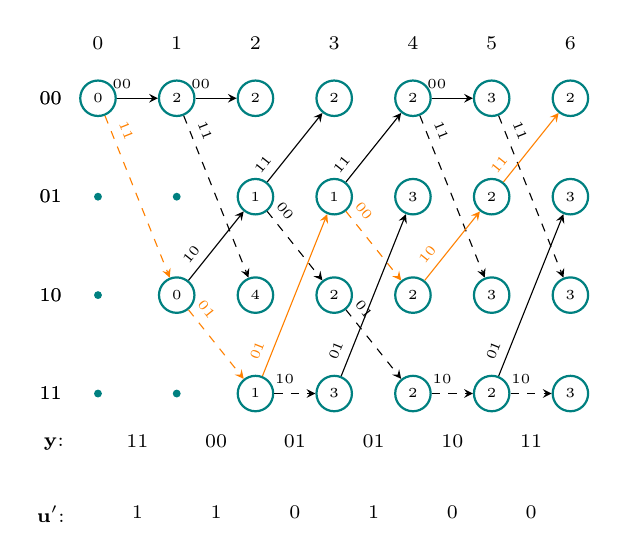
\begin{tikzpicture}[>=stealth, font=\scriptsize]
\tikzstyle{state} = [draw, circle, teal, thick, text=black, minimum size=4.5mm, inner sep=0mm, font=\tiny]
\tikzstyle{freestate} = [circle, teal, fill=teal, minimum size=1mm, inner sep=0mm]

\node[state] (node00) at (0,0) {0} ; 
\node[freestate] (node10) at (0,-1.25) {} ; 
\node[freestate] (node20) at (0,-2.5) {} ; 
\node[freestate] (node30) at (0,-3.75) {} ; 

\node[state] (node01) at (1,0) {2} ; 
\node[freestate] (node11) at (1,-1.25) {} ; 
\node[state] (node21) at (1,-2.5) {0} ; 
\node[freestate] (node31) at (1,-3.75) {} ; 

\node[state] (node02) at (2,0) {2} ; 
\node[state] (node12) at (2,-1.25) {1} ; 
\node[state] (node22) at (2,-2.5) {4} ; 
\node[state] (node32) at (2,-3.75) {1} ; 

\node[state] (node03) at (3,0) {2} ; 
\node[state] (node13) at (3,-1.25) {1} ; 
\node[state] (node23) at (3,-2.5) {2} ; 
\node[state] (node33) at (3,-3.75) {3} ; 

\node[state] (node04) at (4,0) {2} ; 
\node[state] (node14) at (4,-1.25) {3} ; 
\node[state] (node24) at (4,-2.5) {2} ; 
\node[state] (node34) at (4,-3.75) {2} ; 

\node[state] (node05) at (5,0) {3} ; 
\node[state] (node15) at (5,-1.25) {2} ; 
\node[state] (node25) at (5,-2.5) {3} ; 
\node[state] (node35) at (5,-3.75) {2} ; 

\node[state] (node06) at (6,0) {2} ; 
\node[state] (node16) at (6,-1.25) {3} ; 
\node[state] (node26) at (6,-2.5) {3} ; 
\node[state] (node36) at (6,-3.75) {3} ; 
\node (statelabel0) [left of=node00, xshift=4mm] {00}; 
\node (statelabel1) [left of=node10, xshift=4mm] {01}; 
\node (statelabel2) [left of=node20, xshift=4mm] {10}; 
\node (statelabel3) [left of=node30, xshift=4mm] {11};

\foreach \x in {0,...,6}
	\node (timelabel\x) [above of=node0\x, yshift=-3mm] {\x};
		
\node (statelabel0) [left of=node00, xshift=4mm] {00}; 
\node (statelabel1) [left of=node10, xshift=4mm] {01}; 
\node (statelabel2) [left of=node20, xshift=4mm] {10}; 
\node (statelabel3) [left of=node30, xshift=4mm] {11};

%t=0
\draw[->] (node00) -- (node01) node [sloped, above, very near start, font=\tiny] {00};
\draw[->, dashed, orange] (node00) -- (node21) node [sloped, above, very near start, font=\tiny] {11};

%t=1
\draw[->] (node01) -- (node02) node [sloped, above, very near start, font=\tiny] {00};
\draw[->, dashed] (node01) -- (node22) node [sloped, above, very near start, font=\tiny] {11};
\draw[->] (node21) -- (node12) node [sloped, above, near start, font=\tiny] {10};
\draw[->, dashed, orange] (node21) -- (node32) node [sloped, above, very near start, font=\tiny] {01};

%t=2
%\draw[->, lightgray] (node02) -- (node03) node [sloped, above, very near start, font=\tiny] {00};
%\draw[->, dashed, lightgray] (node02) -- (node23) node [sloped, above, very near start, font=\tiny] {11};
\draw[->] (node12) -- (node03) node [sloped, above, very near start, font=\tiny] {11};
\draw[->, dashed] (node12) -- (node23) node [sloped, above, very near start, font=\tiny] {00};
%\draw[->, lightgray] (node22) -- (node13) node [sloped, above, near start, font=\tiny] {10};
%\draw[->, dashed, lightgray] (node22) -- (node33) node [sloped, above, very near start, font=\tiny] {01};
\draw[->, orange] (node32) -- (node13) node [sloped, above, very near start, font=\tiny] {01};
\draw[->, dashed] (node32) -- (node33) node [sloped, above, near start, font=\tiny] {10};

%t=3
%\draw[->, lightgray] (node03) -- (node04) node [sloped, above, very near start, font=\tiny] {00};
%\draw[->, dashed, lightgray] (node03) -- (node24) node [sloped, above, very near start, font=\tiny] {11};
\draw[->] (node13) -- (node04) node [sloped, above, very near start, font=\tiny] {11};
\draw[->, dashed, orange] (node13) -- (node24) node [sloped, above, very near start, font=\tiny] {00};
%\draw[->, lightgray] (node23) -- (node14) node [sloped, above, near start, font=\tiny] {10};
\draw[->, dashed] (node23) -- (node34) node [sloped, above, very near start, font=\tiny] {01};
\draw[->] (node33) -- (node14) node [sloped, above, very near start, font=\tiny] {01};
%\draw[->, dashed, lightgray] (node33) -- (node34) node [sloped, above, near start, font=\tiny] {10};

%t=4
\draw[->] (node04) -- (node05) node [sloped, above, very near start, font=\tiny] {00};
\draw[->, dashed] (node04) -- (node25) node [sloped, above, very near start, font=\tiny] {11};
%\draw[->, lightgray] (node14) -- (node05) node [sloped, above, very near start, font=\tiny] {11};
%\draw[->, dashed, lightgray] (node14) -- (node25) node [sloped, above, very near start, font=\tiny] {00};
\draw[->,orange] (node24) -- (node15) node [sloped, above, near start, font=\tiny] {10};
%\draw[->, dashed, lightgray] (node24) -- (node35) node [sloped, above, very near start, font=\tiny] {01};
%\draw[->, lightgray] (node34) -- (node15) node [sloped, above, very near start, font=\tiny] {01};
\draw[->, dashed] (node34) -- (node35) node [sloped, above, near start, font=\tiny] {10};

%t=5
%\draw[->, lightgray] (node05) -- (node06) node [sloped, above, very near start, font=\tiny] {00};
\draw[->, dashed] (node05) -- (node26) node [sloped, above, very near start, font=\tiny] {11};
\draw[->,orange] (node15) -- (node06) node [sloped, above, very near start, font=\tiny] {11};
%\draw[->, dashed, lightgray] (node15) -- (node26) node [sloped, above, very near start, font=\tiny] {00};
%\draw[->, lightgray] (node25) -- (node16) node [sloped, above, near start, font=\tiny] {10};
%\draw[->, dashed, lightgray] (node25) -- (node36) node [sloped, above, very near start, font=\tiny] {01};
\draw[->] (node35) -- (node16) node [sloped, above, very near start, font=\tiny] {01};
\draw[->, dashed] (node35) -- (node36) node [sloped, above, near start, font=\tiny] {10};

% input & output
\node (in0) at($(node30)!0.5!(node31)+(0,-.6)$) {11};
\node (in1) at($(node31)!0.5!(node32)+(0,-.6)$) {00};
\node (in2) at($(node32)!0.5!(node33)+(0,-.6)$) {01};
\node (in3) at($(node33)!0.5!(node34)+(0,-.6)$) {01};
\node (in4) at($(node34)!0.5!(node35)+(0,-.6)$) {10};
\node (in5) at($(node35)!0.5!(node36)+(0,-.6)$) {11};
\node (inlabel) at($(node30)+(-.56,-.64)$) {$\mathbf{y}$:};

\node (out0) [below=of in0, yshift=5mm] {1};
\node (out1) [below=of in1, yshift=5mm] {1};
\node (out2) [below=of in2, yshift=5mm] {0};
\node (out3) [below=of in3, yshift=5mm] {1};
\node (out4) [below=of in4, yshift=5mm] {0};
\node (out5) [below=of in5, yshift=5mm] {0};
\node (outlabel) at($(node30)+(-.6,-1.53)$) {$\mathbf{u'}$:};

\end{tikzpicture}
	}
	\caption{Backtracking im Trellis der hard decision Dekodierung zu Beispiel~\ref{bsp:B3}}
	\label{abb:trellis_dek_hard_b}
\end{figure}

%\begin{figure}[t]
%	\centering
%	\resizebox{\textwidth}{!}{%
%		\begin{subfigure}[t]{0.42\textwidth}
%			\centering
%			\resizebox{0.99\textwidth}{!}{%
%				\input{tikz/trellis_dekodierung_hard1}
%			}
%			\caption{}
%			\label{abb:trellis_dek_hard_a}
%		\end{subfigure}
%		\begin{subfigure}[t]{0.42\textwidth}
%			\centering
%			\resizebox{0.99\textwidth}{!}{%
%				% trellis_dekodierung_hard2.tex
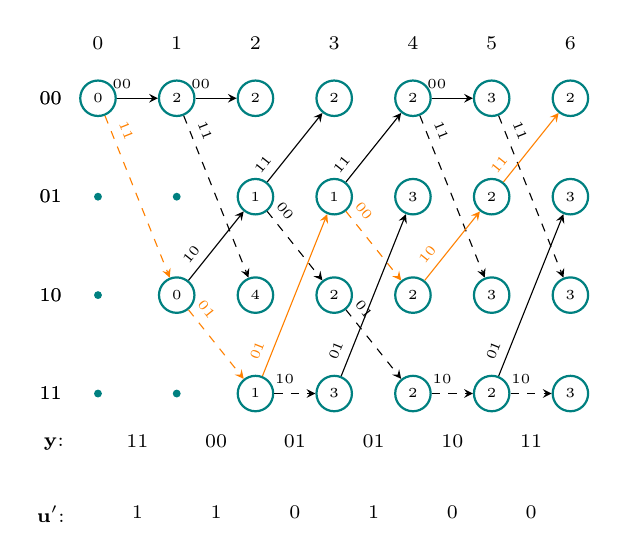
\begin{tikzpicture}[>=stealth, font=\scriptsize]
\tikzstyle{state} = [draw, circle, teal, thick, text=black, minimum size=4.5mm, inner sep=0mm, font=\tiny]
\tikzstyle{freestate} = [circle, teal, fill=teal, minimum size=1mm, inner sep=0mm]

\node[state] (node00) at (0,0) {0} ; 
\node[freestate] (node10) at (0,-1.25) {} ; 
\node[freestate] (node20) at (0,-2.5) {} ; 
\node[freestate] (node30) at (0,-3.75) {} ; 

\node[state] (node01) at (1,0) {2} ; 
\node[freestate] (node11) at (1,-1.25) {} ; 
\node[state] (node21) at (1,-2.5) {0} ; 
\node[freestate] (node31) at (1,-3.75) {} ; 

\node[state] (node02) at (2,0) {2} ; 
\node[state] (node12) at (2,-1.25) {1} ; 
\node[state] (node22) at (2,-2.5) {4} ; 
\node[state] (node32) at (2,-3.75) {1} ; 

\node[state] (node03) at (3,0) {2} ; 
\node[state] (node13) at (3,-1.25) {1} ; 
\node[state] (node23) at (3,-2.5) {2} ; 
\node[state] (node33) at (3,-3.75) {3} ; 

\node[state] (node04) at (4,0) {2} ; 
\node[state] (node14) at (4,-1.25) {3} ; 
\node[state] (node24) at (4,-2.5) {2} ; 
\node[state] (node34) at (4,-3.75) {2} ; 

\node[state] (node05) at (5,0) {3} ; 
\node[state] (node15) at (5,-1.25) {2} ; 
\node[state] (node25) at (5,-2.5) {3} ; 
\node[state] (node35) at (5,-3.75) {2} ; 

\node[state] (node06) at (6,0) {2} ; 
\node[state] (node16) at (6,-1.25) {3} ; 
\node[state] (node26) at (6,-2.5) {3} ; 
\node[state] (node36) at (6,-3.75) {3} ; 
\node (statelabel0) [left of=node00, xshift=4mm] {00}; 
\node (statelabel1) [left of=node10, xshift=4mm] {01}; 
\node (statelabel2) [left of=node20, xshift=4mm] {10}; 
\node (statelabel3) [left of=node30, xshift=4mm] {11};

\foreach \x in {0,...,6}
	\node (timelabel\x) [above of=node0\x, yshift=-3mm] {\x};
		
\node (statelabel0) [left of=node00, xshift=4mm] {00}; 
\node (statelabel1) [left of=node10, xshift=4mm] {01}; 
\node (statelabel2) [left of=node20, xshift=4mm] {10}; 
\node (statelabel3) [left of=node30, xshift=4mm] {11};

%t=0
\draw[->] (node00) -- (node01) node [sloped, above, very near start, font=\tiny] {00};
\draw[->, dashed, orange] (node00) -- (node21) node [sloped, above, very near start, font=\tiny] {11};

%t=1
\draw[->] (node01) -- (node02) node [sloped, above, very near start, font=\tiny] {00};
\draw[->, dashed] (node01) -- (node22) node [sloped, above, very near start, font=\tiny] {11};
\draw[->] (node21) -- (node12) node [sloped, above, near start, font=\tiny] {10};
\draw[->, dashed, orange] (node21) -- (node32) node [sloped, above, very near start, font=\tiny] {01};

%t=2
%\draw[->, lightgray] (node02) -- (node03) node [sloped, above, very near start, font=\tiny] {00};
%\draw[->, dashed, lightgray] (node02) -- (node23) node [sloped, above, very near start, font=\tiny] {11};
\draw[->] (node12) -- (node03) node [sloped, above, very near start, font=\tiny] {11};
\draw[->, dashed] (node12) -- (node23) node [sloped, above, very near start, font=\tiny] {00};
%\draw[->, lightgray] (node22) -- (node13) node [sloped, above, near start, font=\tiny] {10};
%\draw[->, dashed, lightgray] (node22) -- (node33) node [sloped, above, very near start, font=\tiny] {01};
\draw[->, orange] (node32) -- (node13) node [sloped, above, very near start, font=\tiny] {01};
\draw[->, dashed] (node32) -- (node33) node [sloped, above, near start, font=\tiny] {10};

%t=3
%\draw[->, lightgray] (node03) -- (node04) node [sloped, above, very near start, font=\tiny] {00};
%\draw[->, dashed, lightgray] (node03) -- (node24) node [sloped, above, very near start, font=\tiny] {11};
\draw[->] (node13) -- (node04) node [sloped, above, very near start, font=\tiny] {11};
\draw[->, dashed, orange] (node13) -- (node24) node [sloped, above, very near start, font=\tiny] {00};
%\draw[->, lightgray] (node23) -- (node14) node [sloped, above, near start, font=\tiny] {10};
\draw[->, dashed] (node23) -- (node34) node [sloped, above, very near start, font=\tiny] {01};
\draw[->] (node33) -- (node14) node [sloped, above, very near start, font=\tiny] {01};
%\draw[->, dashed, lightgray] (node33) -- (node34) node [sloped, above, near start, font=\tiny] {10};

%t=4
\draw[->] (node04) -- (node05) node [sloped, above, very near start, font=\tiny] {00};
\draw[->, dashed] (node04) -- (node25) node [sloped, above, very near start, font=\tiny] {11};
%\draw[->, lightgray] (node14) -- (node05) node [sloped, above, very near start, font=\tiny] {11};
%\draw[->, dashed, lightgray] (node14) -- (node25) node [sloped, above, very near start, font=\tiny] {00};
\draw[->,orange] (node24) -- (node15) node [sloped, above, near start, font=\tiny] {10};
%\draw[->, dashed, lightgray] (node24) -- (node35) node [sloped, above, very near start, font=\tiny] {01};
%\draw[->, lightgray] (node34) -- (node15) node [sloped, above, very near start, font=\tiny] {01};
\draw[->, dashed] (node34) -- (node35) node [sloped, above, near start, font=\tiny] {10};

%t=5
%\draw[->, lightgray] (node05) -- (node06) node [sloped, above, very near start, font=\tiny] {00};
\draw[->, dashed] (node05) -- (node26) node [sloped, above, very near start, font=\tiny] {11};
\draw[->,orange] (node15) -- (node06) node [sloped, above, very near start, font=\tiny] {11};
%\draw[->, dashed, lightgray] (node15) -- (node26) node [sloped, above, very near start, font=\tiny] {00};
%\draw[->, lightgray] (node25) -- (node16) node [sloped, above, near start, font=\tiny] {10};
%\draw[->, dashed, lightgray] (node25) -- (node36) node [sloped, above, very near start, font=\tiny] {01};
\draw[->] (node35) -- (node16) node [sloped, above, very near start, font=\tiny] {01};
\draw[->, dashed] (node35) -- (node36) node [sloped, above, near start, font=\tiny] {10};

% input & output
\node (in0) at($(node30)!0.5!(node31)+(0,-.6)$) {11};
\node (in1) at($(node31)!0.5!(node32)+(0,-.6)$) {00};
\node (in2) at($(node32)!0.5!(node33)+(0,-.6)$) {01};
\node (in3) at($(node33)!0.5!(node34)+(0,-.6)$) {01};
\node (in4) at($(node34)!0.5!(node35)+(0,-.6)$) {10};
\node (in5) at($(node35)!0.5!(node36)+(0,-.6)$) {11};
\node (inlabel) at($(node30)+(-.56,-.64)$) {$\mathbf{y}$:};

\node (out0) [below=of in0, yshift=5mm] {1};
\node (out1) [below=of in1, yshift=5mm] {1};
\node (out2) [below=of in2, yshift=5mm] {0};
\node (out3) [below=of in3, yshift=5mm] {1};
\node (out4) [below=of in4, yshift=5mm] {0};
\node (out5) [below=of in5, yshift=5mm] {0};
\node (outlabel) at($(node30)+(-.6,-1.53)$) {$\mathbf{u'}$:};

\end{tikzpicture}
%			}
%			\caption{}
%			\label{abb:trellis_dek_hard_b}
%		\end{subfigure}
%	}
%	\caption{Trellis der hard decision Dekodierung zu Beispiel~\ref{bsp:B3}}
%	\label{abb:trellis_dekodierung_hard}
%\end{figure}

\subsubsection{soft decision}
\label{kapitel:grundlagen_soft_decision}
Vor der Übertragung eines Kodeworts werden die Kodebits 0 bzw. 1 nach Gleichung~\eqref{eq:bit_zu_signal_abbildung} auf die Signalzustände +1 bzw. -1 abgebildet. Bei der hard decision Dekodierung muss vor der Dekodierung das Signal nach Gleichung~\eqref{eq:signal_zu_bit_abbildung} wieder zu einem Bitvektor zurück umgewandelt werden. Die soft decision Dekodierung lässt diese Rücktransformation aus und verwendet die exakten Signalpegel. Dadurch erzielt die soft decision Dekodierung eine noch bessere Fehlerkorrektur. Die Metrik für eine Kante, die einen Zustand $s$ zum Zeitpunkt $t$ mit einem Zustand $s'$ zum Zeitpunkt $t+1$ verbindet, entspricht dem Skalarprodukt der Signalzustände der Bewertung der Kante zwischen $s$ und $s'$ und dem zum Zeitpunkt $t$ empfangenen Teil des Signals. Der Viterbi-Algorithmus funktioniert analog zur soft decision Dekodierung, jedoch wird der Pfad mit der maximalen Metrik gesucht. Treffen zwei Pfade aufeinander, wird der Pfad mit der kleineren Metrik verworfen. Das Backtracking beginnt hier bei der größten Metrik. Als Ergebnis resultiert die Nachricht, dessen Signal das größte Skalarprodukt mit dem empfangenen Signal hat.
\\
\\
Die Nachricht wird mittels \emph{Soft-Werten} und \emph{Hard-Werten} angegeben. Die Soft-Werte geben neben der dekodierten Nachricht die Zuverlässigkeitswerte für die Bits an, d.h. mit welcher Wahrscheinlichkeit das Bit mit dem tatsächlich gesendeten Bit der Quellnachricht übereinstimmt. Positive Soft-Werte werden auf eine 0, negative auf eine 1 abgebildet. Der Betrag des Soft-Werts gibt die Zuverlässigkeit an, wobei gilt, je höher der Betrag, desto zuverlässiger das dekodierte Bit. Die Hard-Werte entsprechen der Abbildung der Soft-Werte auf die Bit-Werte 0 bzw. 1. Der Viterbi-Algorithmus mit Soft-Werten wird auch SOVA (Soft Output Viterbi Algorithm) genannt. Die Berechnung der Soft-Werte ist in \cite[S.~228~ff.]{schonfeld2012informations} beschrieben.

\begin{beispiel}
Gegeben sei der Faltungskodierer aus Beispiel~\ref{bsp:B1} und ein empfangenes Signal $\mathbf{y}=\left( -1~-1~~0.5~-1~~0.9~-0.9~~1~-0.2~~-0.8~-0.1~-1~-1\right)$, welches durch Rauschen verfälscht wurde und dekodiert werden soll. Abbildung~\ref{abb:trellis_dek_soft_a} zeigt die Dekodierung im Trellis mit den Metriken aller Pfade. Die verworfenen Pfade sind grau dargestellt. Beispielsweise ergibt sich die Metrik zum Zeitpunkt 1 im Zustand 00 durch $0+\left( 1\cdot\left( -1\right) + 1\cdot\left( -1\right)\right) =0-2=-2$, im Zustand 10 durch $0+\left( \left( -1\right)\cdot\left( -1\right) + \left( -1\right)\cdot\left( -1\right)\right) =0+2=2$. Der erste Summand entspricht der Metrik des vorigen Zustands. Die Bits der Kantenbewertung im Trellis müssen für die Berechnung des Skalarprodukts auf die Signalzustände +1 bzw. -1 abgebildet werden. In Abbildung~\ref{abb:trellis_dek_soft_b} werden die verworfenen Pfade nicht mehr angezeigt. Aus dem Backtracking resultiert die dekodierte Nachricht $\mathbf{u'}=\left( 110100\right)$. Der Pfad der dekodierten Nachricht im Trellis ist orange hervorgehoben.
\label{bsp:B4}
\end{beispiel}

\begin{figure}[t]
	\centering
	\resizebox{0.70\textwidth}{!}{%
		% trellis_dekodierung_soft1.tex
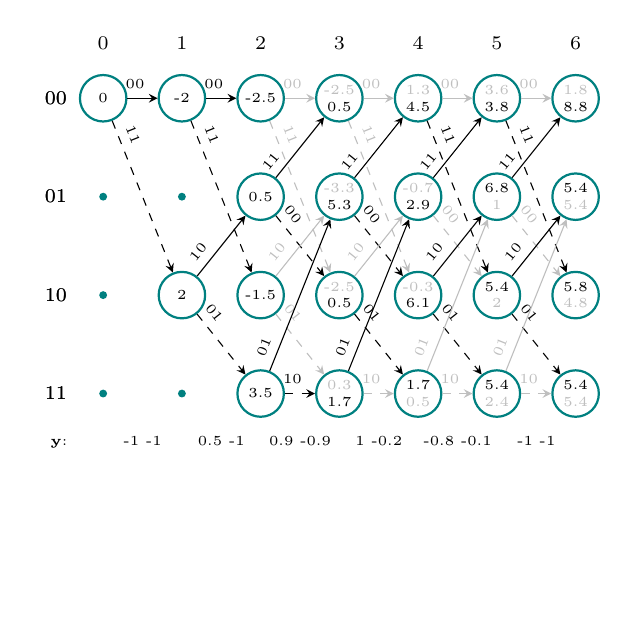
\begin{tikzpicture}[>=stealth, font=\scriptsize]
\tikzstyle{state} = [draw, circle, teal, thick, text=black, minimum size=5.9mm, inner sep=0mm, font=\tiny, align=center]
\tikzstyle{freestate} = [circle, teal, fill=teal, minimum size=1mm, inner sep=0mm]

\node[state] (node00) at (0,0) {0} ; 
\node[freestate] (node10) at (0,-1.25) {} ; 
\node[freestate] (node20) at (0,-2.5) {} ; 
\node[freestate] (node30) at (0,-3.75) {} ; 

\node[state] (node01) at (1,0) {-2} ; 
\node[freestate] (node11) at (1,-1.25) {} ; 
\node[state] (node21) at (1,-2.5) {2} ; 
\node[freestate] (node31) at (1,-3.75) {} ; 

\node[state] (node02) at (2,0) {-2.5} ; 
\node[state] (node12) at (2,-1.25) {0.5} ; 
\node[state] (node22) at (2,-2.5) {-1.5} ; 
\node[state] (node32) at (2,-3.75) {3.5} ; 

\node[state] (node03) at (3,0) {\textcolor{lightgray}{-2.5}\\ \textcolor{black}{0.5}} ; 
\node[state] (node13) at (3,-1.25) {\textcolor{lightgray}{-3.3}\\ \textcolor{black}{5.3}} ; 
\node[state] (node23) at (3,-2.5) {\textcolor{lightgray}{-2.5}\\ \textcolor{black}{0.5}} ; 
\node[state] (node33) at (3,-3.75) {\textcolor{lightgray}{0.3}\\ \textcolor{black}{1.7}} ; 

\node[state] (node04) at (4,0) {\textcolor{lightgray}{1.3}\\ \textcolor{black}{4.5}} ; 
\node[state] (node14) at (4,-1.25) {\textcolor{lightgray}{-0.7}\\ \textcolor{black}{2.9}} ; 
\node[state] (node24) at (4,-2.5) {\textcolor{lightgray}{-0.3}\\ \textcolor{black}{6.1}} ; 
\node[state] (node34) at (4,-3.75) {1.7\\ \textcolor{lightgray}{0.5}} ; 

\node[state] (node05) at (5,0) {\textcolor{lightgray}{3.6}\\ \textcolor{black}{3.8}} ; 
\node[state] (node15) at (5,-1.25) {6.8\\ \textcolor{lightgray}{1}} ; 
\node[state] (node25) at (5,-2.5) {5.4\\ \textcolor{lightgray}{2}} ; 
\node[state] (node35) at (5,-3.75) {5.4\\ \textcolor{lightgray}{2.4}} ; 

\node[state] (node06) at (6,0) {\textcolor{lightgray}{1.8}\\ \textcolor{black}{8.8}} ; 
\node[state] (node16) at (6,-1.25) {5.4\\ \textcolor{lightgray}{5.4}} ; 
\node[state] (node26) at (6,-2.5) {5.8\\ \textcolor{lightgray}{4.8}} ; 
\node[state] (node36) at (6,-3.75) {5.4\\ \textcolor{lightgray}{5.4}} ; 
\node (statelabel0) [left of=node00, xshift=4mm] {00}; 
\node (statelabel1) [left of=node10, xshift=4mm] {01}; 
\node (statelabel2) [left of=node20, xshift=4mm] {10}; 
\node (statelabel3) [left of=node30, xshift=4mm] {11};

\foreach \x in {0,...,6}
	\node (timelabel\x) [above of=node0\x, yshift=-3mm] {\x};
		
\node (statelabel0) [left of=node00, xshift=4mm] {00}; 
\node (statelabel1) [left of=node10, xshift=4mm] {01}; 
\node (statelabel2) [left of=node20, xshift=4mm] {10}; 
\node (statelabel3) [left of=node30, xshift=4mm] {11};

%t=0
\draw[->] (node00) -- (node01) node [sloped, above, near start, font=\tiny] {00};
\draw[->, dashed] (node00) -- (node21) node [sloped, above, very near start, font=\tiny] {11};

%t=1
\draw[->] (node01) -- (node02) node [sloped, above, near start, font=\tiny] {00};
\draw[->, dashed] (node01) -- (node22) node [sloped, above, very near start, font=\tiny] {11};
\draw[->] (node21) -- (node12) node [sloped, above, near start, font=\tiny] {10};
\draw[->, dashed] (node21) -- (node32) node [sloped, above, very near start, font=\tiny] {01};

%t=2
\draw[->, lightgray] (node02) -- (node03) node [sloped, above, near start, font=\tiny] {00};
\draw[->, dashed, lightgray] (node02) -- (node23) node [sloped, above, very near start, font=\tiny] {11};
\draw[->] (node12) -- (node03) node [sloped, above, very near start, font=\tiny] {11};
\draw[->, dashed] (node12) -- (node23) node [sloped, above, very near start, font=\tiny] {00};
\draw[->, lightgray] (node22) -- (node13) node [sloped, above, near start, font=\tiny] {10};
\draw[->, dashed, lightgray] (node22) -- (node33) node [sloped, above, very near start, font=\tiny] {01};
\draw[->] (node32) -- (node13) node [sloped, above, very near start, font=\tiny] {01};
\draw[->, dashed] (node32) -- (node33) node [sloped, above, near start, font=\tiny] {10};

%t=3
\draw[->, lightgray] (node03) -- (node04) node [sloped, above, near start, font=\tiny] {00};
\draw[->, dashed, lightgray] (node03) -- (node24) node [sloped, above, very near start, font=\tiny] {11};
\draw[->] (node13) -- (node04) node [sloped, above, very near start, font=\tiny] {11};
\draw[->, dashed] (node13) -- (node24) node [sloped, above, very near start, font=\tiny] {00};
\draw[->, lightgray] (node23) -- (node14) node [sloped, above, near start, font=\tiny] {10};
\draw[->, dashed] (node23) -- (node34) node [sloped, above, very near start, font=\tiny] {01};
\draw[->] (node33) -- (node14) node [sloped, above, very near start, font=\tiny] {01};
\draw[->, dashed, lightgray] (node33) -- (node34) node [sloped, above, near start, font=\tiny] {10};

%t=4
\draw[->, lightgray] (node04) -- (node05) node [sloped, above, near start, font=\tiny] {00};
\draw[->, dashed] (node04) -- (node25) node [sloped, above, very near start, font=\tiny] {11};
\draw[->] (node14) -- (node05) node [sloped, above, very near start, font=\tiny] {11};
\draw[->, dashed, lightgray] (node14) -- (node25) node [sloped, above, very near start, font=\tiny] {00};
\draw[->] (node24) -- (node15) node [sloped, above, near start, font=\tiny] {10};
\draw[->, dashed] (node24) -- (node35) node [sloped, above, very near start, font=\tiny] {01};
\draw[->, lightgray] (node34) -- (node15) node [sloped, above, very near start, font=\tiny] {01};
\draw[->, dashed, lightgray] (node34) -- (node35) node [sloped, above, near start, font=\tiny] {10};

%t=5
\draw[->, lightgray] (node05) -- (node06) node [sloped, above, near start, font=\tiny] {00};
\draw[->, dashed] (node05) -- (node26) node [sloped, above, very near start, font=\tiny] {11};
\draw[->] (node15) -- (node06) node [sloped, above, very near start, font=\tiny] {11};
\draw[->, dashed, lightgray] (node15) -- (node26) node [sloped, above, very near start, font=\tiny] {00};
\draw[->] (node25) -- (node16) node [sloped, above, near start, font=\tiny] {10};
\draw[->, dashed] (node25) -- (node36) node [sloped, above, very near start, font=\tiny] {01};
\draw[->, lightgray] (node35) -- (node16) node [sloped, above, very near start, font=\tiny] {01};
\draw[->, dashed, lightgray] (node35) -- (node36) node [sloped, above, near start, font=\tiny] {10};

% input & output
\node[font=\tiny] (in0) at($(node30)!0.5!(node31)+(0,-.6)$) {-1~-1};
\node[font=\tiny] (in1) at($(node31)!0.5!(node32)+(0,-.6)$) {0.5~-1};
\node[font=\tiny] (in2) at($(node32)!0.5!(node33)+(0,-.6)$) {0.9~-0.9};
\node[font=\tiny] (in3) at($(node33)!0.5!(node34)+(0,-.6)$) {1~-0.2};
\node[font=\tiny] (in4) at($(node34)!0.5!(node35)+(0,-.6)$) {-0.8~-0.1};
\node[font=\tiny] (in5) at($(node35)!0.5!(node36)+(0,-.6)$) {-1~-1};
\node[font=\tiny] (inlabel) at($(node30)+(-.56,-.64)$) {$\mathbf{y}$:};

\node[font=\tiny] (out0) [below=of in0, yshift=5mm] {\textcolor{white}{-4.3}};
\node[font=\tiny] (out1) [below=of in1, yshift=5mm] {\textcolor{white}{-2.9}};
\node[font=\tiny] (out2) [below=of in2, yshift=5mm] {\textcolor{white}{2.9}};
\node[font=\tiny] (out3) [below=of in3, yshift=5mm] {\textcolor{white}{-2.9}};
\node[font=\tiny] (out4) [below=of in4, yshift=5mm] {\textcolor{white}{2.9}};
\node[font=\tiny] (out5) [below=of in5, yshift=5mm] {\textcolor{white}{3.5}};
\node[font=\tiny] (outlabel) at($(node30)+(-.65,-1.53)$) {\textcolor{white}{$\mathbf{u'_{s}}$:}};

\node[font=\tiny] [below=of out0, yshift=5mm] {\textcolor{white}{1}};
\node[font=\tiny] [below=of out1, yshift=5mm] {\textcolor{white}{1}};
\node[font=\tiny] [below=of out2, yshift=5mm] {\textcolor{white}{0}};
\node[font=\tiny] [below=of out3, yshift=5mm] {\textcolor{white}{1}};
\node[font=\tiny] [below=of out4, yshift=5mm] {\textcolor{white}{0}};
\node[font=\tiny] [below=of out5, yshift=5mm] {\textcolor{white}{0}};
\node[font=\tiny] at($(node30)+(-.65,-2.43)$) {\textcolor{white}{$\mathbf{u'_{h}}$:}};

\end{tikzpicture}
	}
	\caption{Vollständiges Trellis der soft decision Dekodierung zu Beispiel~\ref{bsp:B4}}
	\label{abb:trellis_dek_soft_a}
\end{figure}
\begin{figure}[t]
	\centering
	\resizebox{0.70\textwidth}{!}{%
		\input{tikz/trellis_dekodierung_soft2}
	}
	\caption{Backtracking im Trellis der hard decision Dekodierung zu Beispiel~\ref{bsp:B4}}
	\label{abb:trellis_dek_soft_b}
\end{figure}

%\begin{figure}[t]
%	\centering
%	\resizebox{\textwidth}{!}{%
%		\begin{subfigure}[t]{0.42\textwidth}
%			\centering
%			\resizebox{0.99\textwidth}{!}{%
%				% trellis_dekodierung_soft1.tex
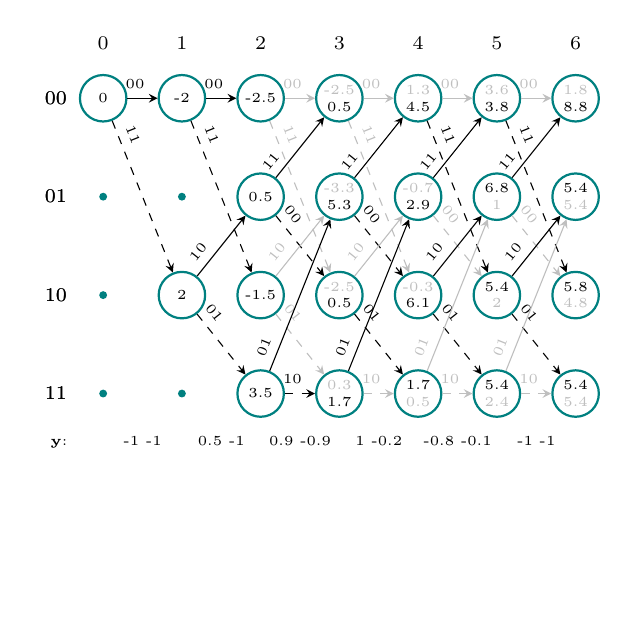
\begin{tikzpicture}[>=stealth, font=\scriptsize]
\tikzstyle{state} = [draw, circle, teal, thick, text=black, minimum size=5.9mm, inner sep=0mm, font=\tiny, align=center]
\tikzstyle{freestate} = [circle, teal, fill=teal, minimum size=1mm, inner sep=0mm]

\node[state] (node00) at (0,0) {0} ; 
\node[freestate] (node10) at (0,-1.25) {} ; 
\node[freestate] (node20) at (0,-2.5) {} ; 
\node[freestate] (node30) at (0,-3.75) {} ; 

\node[state] (node01) at (1,0) {-2} ; 
\node[freestate] (node11) at (1,-1.25) {} ; 
\node[state] (node21) at (1,-2.5) {2} ; 
\node[freestate] (node31) at (1,-3.75) {} ; 

\node[state] (node02) at (2,0) {-2.5} ; 
\node[state] (node12) at (2,-1.25) {0.5} ; 
\node[state] (node22) at (2,-2.5) {-1.5} ; 
\node[state] (node32) at (2,-3.75) {3.5} ; 

\node[state] (node03) at (3,0) {\textcolor{lightgray}{-2.5}\\ \textcolor{black}{0.5}} ; 
\node[state] (node13) at (3,-1.25) {\textcolor{lightgray}{-3.3}\\ \textcolor{black}{5.3}} ; 
\node[state] (node23) at (3,-2.5) {\textcolor{lightgray}{-2.5}\\ \textcolor{black}{0.5}} ; 
\node[state] (node33) at (3,-3.75) {\textcolor{lightgray}{0.3}\\ \textcolor{black}{1.7}} ; 

\node[state] (node04) at (4,0) {\textcolor{lightgray}{1.3}\\ \textcolor{black}{4.5}} ; 
\node[state] (node14) at (4,-1.25) {\textcolor{lightgray}{-0.7}\\ \textcolor{black}{2.9}} ; 
\node[state] (node24) at (4,-2.5) {\textcolor{lightgray}{-0.3}\\ \textcolor{black}{6.1}} ; 
\node[state] (node34) at (4,-3.75) {1.7\\ \textcolor{lightgray}{0.5}} ; 

\node[state] (node05) at (5,0) {\textcolor{lightgray}{3.6}\\ \textcolor{black}{3.8}} ; 
\node[state] (node15) at (5,-1.25) {6.8\\ \textcolor{lightgray}{1}} ; 
\node[state] (node25) at (5,-2.5) {5.4\\ \textcolor{lightgray}{2}} ; 
\node[state] (node35) at (5,-3.75) {5.4\\ \textcolor{lightgray}{2.4}} ; 

\node[state] (node06) at (6,0) {\textcolor{lightgray}{1.8}\\ \textcolor{black}{8.8}} ; 
\node[state] (node16) at (6,-1.25) {5.4\\ \textcolor{lightgray}{5.4}} ; 
\node[state] (node26) at (6,-2.5) {5.8\\ \textcolor{lightgray}{4.8}} ; 
\node[state] (node36) at (6,-3.75) {5.4\\ \textcolor{lightgray}{5.4}} ; 
\node (statelabel0) [left of=node00, xshift=4mm] {00}; 
\node (statelabel1) [left of=node10, xshift=4mm] {01}; 
\node (statelabel2) [left of=node20, xshift=4mm] {10}; 
\node (statelabel3) [left of=node30, xshift=4mm] {11};

\foreach \x in {0,...,6}
	\node (timelabel\x) [above of=node0\x, yshift=-3mm] {\x};
		
\node (statelabel0) [left of=node00, xshift=4mm] {00}; 
\node (statelabel1) [left of=node10, xshift=4mm] {01}; 
\node (statelabel2) [left of=node20, xshift=4mm] {10}; 
\node (statelabel3) [left of=node30, xshift=4mm] {11};

%t=0
\draw[->] (node00) -- (node01) node [sloped, above, near start, font=\tiny] {00};
\draw[->, dashed] (node00) -- (node21) node [sloped, above, very near start, font=\tiny] {11};

%t=1
\draw[->] (node01) -- (node02) node [sloped, above, near start, font=\tiny] {00};
\draw[->, dashed] (node01) -- (node22) node [sloped, above, very near start, font=\tiny] {11};
\draw[->] (node21) -- (node12) node [sloped, above, near start, font=\tiny] {10};
\draw[->, dashed] (node21) -- (node32) node [sloped, above, very near start, font=\tiny] {01};

%t=2
\draw[->, lightgray] (node02) -- (node03) node [sloped, above, near start, font=\tiny] {00};
\draw[->, dashed, lightgray] (node02) -- (node23) node [sloped, above, very near start, font=\tiny] {11};
\draw[->] (node12) -- (node03) node [sloped, above, very near start, font=\tiny] {11};
\draw[->, dashed] (node12) -- (node23) node [sloped, above, very near start, font=\tiny] {00};
\draw[->, lightgray] (node22) -- (node13) node [sloped, above, near start, font=\tiny] {10};
\draw[->, dashed, lightgray] (node22) -- (node33) node [sloped, above, very near start, font=\tiny] {01};
\draw[->] (node32) -- (node13) node [sloped, above, very near start, font=\tiny] {01};
\draw[->, dashed] (node32) -- (node33) node [sloped, above, near start, font=\tiny] {10};

%t=3
\draw[->, lightgray] (node03) -- (node04) node [sloped, above, near start, font=\tiny] {00};
\draw[->, dashed, lightgray] (node03) -- (node24) node [sloped, above, very near start, font=\tiny] {11};
\draw[->] (node13) -- (node04) node [sloped, above, very near start, font=\tiny] {11};
\draw[->, dashed] (node13) -- (node24) node [sloped, above, very near start, font=\tiny] {00};
\draw[->, lightgray] (node23) -- (node14) node [sloped, above, near start, font=\tiny] {10};
\draw[->, dashed] (node23) -- (node34) node [sloped, above, very near start, font=\tiny] {01};
\draw[->] (node33) -- (node14) node [sloped, above, very near start, font=\tiny] {01};
\draw[->, dashed, lightgray] (node33) -- (node34) node [sloped, above, near start, font=\tiny] {10};

%t=4
\draw[->, lightgray] (node04) -- (node05) node [sloped, above, near start, font=\tiny] {00};
\draw[->, dashed] (node04) -- (node25) node [sloped, above, very near start, font=\tiny] {11};
\draw[->] (node14) -- (node05) node [sloped, above, very near start, font=\tiny] {11};
\draw[->, dashed, lightgray] (node14) -- (node25) node [sloped, above, very near start, font=\tiny] {00};
\draw[->] (node24) -- (node15) node [sloped, above, near start, font=\tiny] {10};
\draw[->, dashed] (node24) -- (node35) node [sloped, above, very near start, font=\tiny] {01};
\draw[->, lightgray] (node34) -- (node15) node [sloped, above, very near start, font=\tiny] {01};
\draw[->, dashed, lightgray] (node34) -- (node35) node [sloped, above, near start, font=\tiny] {10};

%t=5
\draw[->, lightgray] (node05) -- (node06) node [sloped, above, near start, font=\tiny] {00};
\draw[->, dashed] (node05) -- (node26) node [sloped, above, very near start, font=\tiny] {11};
\draw[->] (node15) -- (node06) node [sloped, above, very near start, font=\tiny] {11};
\draw[->, dashed, lightgray] (node15) -- (node26) node [sloped, above, very near start, font=\tiny] {00};
\draw[->] (node25) -- (node16) node [sloped, above, near start, font=\tiny] {10};
\draw[->, dashed] (node25) -- (node36) node [sloped, above, very near start, font=\tiny] {01};
\draw[->, lightgray] (node35) -- (node16) node [sloped, above, very near start, font=\tiny] {01};
\draw[->, dashed, lightgray] (node35) -- (node36) node [sloped, above, near start, font=\tiny] {10};

% input & output
\node[font=\tiny] (in0) at($(node30)!0.5!(node31)+(0,-.6)$) {-1~-1};
\node[font=\tiny] (in1) at($(node31)!0.5!(node32)+(0,-.6)$) {0.5~-1};
\node[font=\tiny] (in2) at($(node32)!0.5!(node33)+(0,-.6)$) {0.9~-0.9};
\node[font=\tiny] (in3) at($(node33)!0.5!(node34)+(0,-.6)$) {1~-0.2};
\node[font=\tiny] (in4) at($(node34)!0.5!(node35)+(0,-.6)$) {-0.8~-0.1};
\node[font=\tiny] (in5) at($(node35)!0.5!(node36)+(0,-.6)$) {-1~-1};
\node[font=\tiny] (inlabel) at($(node30)+(-.56,-.64)$) {$\mathbf{y}$:};

\node[font=\tiny] (out0) [below=of in0, yshift=5mm] {\textcolor{white}{-4.3}};
\node[font=\tiny] (out1) [below=of in1, yshift=5mm] {\textcolor{white}{-2.9}};
\node[font=\tiny] (out2) [below=of in2, yshift=5mm] {\textcolor{white}{2.9}};
\node[font=\tiny] (out3) [below=of in3, yshift=5mm] {\textcolor{white}{-2.9}};
\node[font=\tiny] (out4) [below=of in4, yshift=5mm] {\textcolor{white}{2.9}};
\node[font=\tiny] (out5) [below=of in5, yshift=5mm] {\textcolor{white}{3.5}};
\node[font=\tiny] (outlabel) at($(node30)+(-.65,-1.53)$) {\textcolor{white}{$\mathbf{u'_{s}}$:}};

\node[font=\tiny] [below=of out0, yshift=5mm] {\textcolor{white}{1}};
\node[font=\tiny] [below=of out1, yshift=5mm] {\textcolor{white}{1}};
\node[font=\tiny] [below=of out2, yshift=5mm] {\textcolor{white}{0}};
\node[font=\tiny] [below=of out3, yshift=5mm] {\textcolor{white}{1}};
\node[font=\tiny] [below=of out4, yshift=5mm] {\textcolor{white}{0}};
\node[font=\tiny] [below=of out5, yshift=5mm] {\textcolor{white}{0}};
\node[font=\tiny] at($(node30)+(-.65,-2.43)$) {\textcolor{white}{$\mathbf{u'_{h}}$:}};

\end{tikzpicture}
%			}
%			\caption{}
%			\label{abb:trellis_dek_soft_a}
%		\end{subfigure}
%		\begin{subfigure}[t]{0.42\textwidth}
%			\centering
%			\resizebox{0.99\textwidth}{!}{%
%				\input{tikz/trellis_dekodierung_soft2}
%			}
%			\caption{}
%			\label{abb:trellis_dek_soft_b}
%		\end{subfigure}
%	}
%	\caption{Trellis der soft decision Dekodierung zu Beispiel~\ref{bsp:B4}}
%	\label{abb:trellis_dekodierung_soft}
%\end{figure}

\subsection{Katastrophale Faltungskodierer}
\label{kapitel:grundlagen_katastrophale_kodierer}
Sei $\mathbf{u}$ eine Nachricht, die mit den Generatorpolynomen in $G$ zum Kode $\mathbf{v}$ kodiert wird. Nach der Übertragung erhält der Dekodierer den Kode $\mathbf{y}$, der aufgrund von Rauschen verändert sein könnte. Der Dekodierer findet ein Kodewort $\mathbf{v'}$ welches $\mathbf{v}$ am nächsten ist. Aus $\mathbf{v'}$ kann die Schätzung $\mathbf{u'}$, die möglichst $\mathbf{u}$ entsprechen sollte, berechnet werden. Dies ist bei einer fehlerfreien Übertragung, d.h. $\mathbf{v'}=\mathbf{v}$, sicherlich der Fall. Im Folgenden wird der Fall $\mathbf{v'}\neq\mathbf{v}$ untersucht: Zu erwarten wäre, wenn sich $\mathbf{v'}$ und $\mathbf{v}$ in endlich vielen Stellen unterscheiden, dass sich auch $\mathbf{u'}$ und $\mathbf{u}$ in endlich vielen Stellen unterscheiden. Wenn sich $\mathbf{u'}$ und $\mathbf{u}$ in unendlich vielen Stellen unterscheiden, wäre das \emph{katastrophal}. Ein Faltungskodierer wird katastrophal genannt, wenn es eine Nachricht mit unendlichem Hamming-Gewicht gibt, sodass sein Kode endliches Hamming-Gewicht hat. Katastrophale Kodierer sind zu vermeiden, da eine endliche Anzahl an Übertragungsfehler zu einer unendlichen Anzahl an Dekodierfehler führen kann.~\cite[S.~569]{huffman2010fundamentals}
\\
\\
Zur Überprüfung, ob ein Kodierer katastrophal ist, hilft das Theorem von Massey-Sain~\cite[S.~570]{huffman2010fundamentals}. Sei ein Faltungskodierer mit einem Eingang und der Generatormatrix $G$ als Polynome über $D$ gegeben. Der Kodierer ist nicht katastrophal genau dann, wenn der größte gemeinsame Teiler der Generatorpolynome eine Potenz von $D$ ist.
\begin{figure}[t]
	\centering
	\begin{subfigure}{0.45\textwidth}
		\centering
		\resizebox{0.90\textwidth}{!}{%
			% systematischer_kodierer.tex
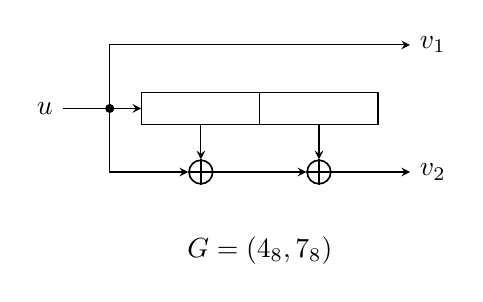
\begin{tikzpicture}[>=stealth]
\tikzstyle{rect} = [draw, rectangle, minimum width=30mm, inner sep=0mm, minimum height=4mm]
\tikzstyle{xor} = [draw, circle, semithick, minimum size=3mm, inner sep=0mm]

\node[rect] (rect) {};
\draw[-] (rect.north) -- (rect.south);
\draw[<-] (rect.west) -- ++(-10mm,0) node [left] {$u$};

\draw[->] ($(rect.west)+(-4mm,0)$) |- ($(rect.north east)+(4mm,6mm)$) node [right] {$v_{1}$};

\node[xor] (xor1) at ($(rect.south)+(-7.5mm,-6mm)$) {};
\draw[semithick] (xor1.north) -- (xor1.south);
\draw[semithick] (xor1.west) -- (xor1.east);
\draw[->] ($(rect.south)+(-7.5mm,0)$) -- (xor1.north);

\node[xor] (xor2) at ($(rect.south)+(7.5mm,-6mm)$) {};
\draw[semithick] (xor2.north) -- (xor2.south);
\draw[semithick] (xor2.west) -- (xor2.east);
\draw[->] ($(rect.south)+(7.5mm,0)$) -- (xor2.north);

\draw[->] ($(rect.west)+(-4mm,0)$) |- (xor1.west);
\draw[->] (xor1.east) -- (xor2.west);
\draw[->] (xor2.east) -- ($(rect.south east)+(4mm,-6mm)$) node [right] {$v_{2}$};
\draw[black, fill=black] ($(rect.west)+(-4mm,0)$) circle [radius=.5mm];

\node at ($(rect.south)+(0,-16mm)$) {$G=\left( 4_{8},7_{8}\right)$};
\end{tikzpicture}
		}
		\caption{Systematischer Faltungskodierer}
		\label{abb:systematischer_kodierer}
	\end{subfigure}
	~ % spacing between subfigures
	\begin{subfigure}{0.45\textwidth}
		\centering
		\resizebox{0.99\textwidth}{!}{%
			% rsc.tex
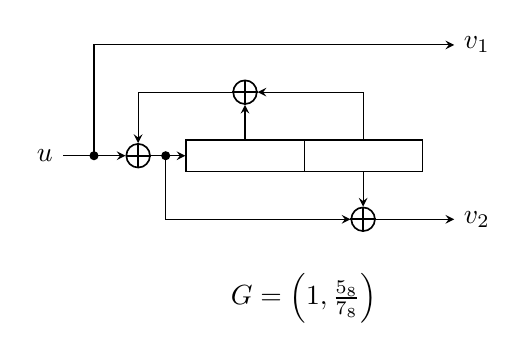
\begin{tikzpicture}[>=stealth]
\tikzstyle{rect} = [draw, rectangle, minimum width=30mm, inner sep=0mm, minimum height=4mm]
\tikzstyle{xor} = [draw, circle, semithick, minimum size=3mm, inner sep=0mm]

\node[rect] (rect) {};
\draw[-] (rect.north) -- (rect.south);

\node[xor] (rec) at ($(rect.west)+(-6mm,0)$) {};
\draw[semithick] (rec.north) -- (rec.south);
\draw[semithick] (rec.west) -- (rec.east);
\node[xor] (xor1) at ($(rect.north)+(-7.5mm,6mm)$) {};
\draw[semithick] (xor1.north) -- (xor1.south);
\draw[semithick] (xor1.west) -- (xor1.east);
\node[xor] (xor2) at ($(rect.south)+(7.5mm,-6mm)$) {};
\draw[semithick] (xor2.north) -- (xor2.south);
\draw[semithick] (xor2.west) -- (xor2.east);

\draw[<-] (rec.west) -- ++(-8mm,0) node [left] {$u$};
\draw[->] (rec.east) -- (rect.west);
\draw[->] ($(rect.north)+(-7.5mm,0)$) -- (xor1.south);
\draw[->] ($(rect.south)+(7.5mm,0)$) -- (xor2.north);
\draw[->] ($(rect.north)+(7.5mm,0)$) |- (xor1.east);
\draw[->] (xor1.west) -| (rec.north);

\draw[->] ($(rect.west)+(-2.5mm,0)$) |- (xor2.west);
\draw[->] (xor2.east) -- ($(rect.south east)+(4mm,-6mm)$) node [right] {$v_{2}$};
\draw[->] ($(rec.west)+(-4mm,0)$) |- ($(rect.north east)+(4mm,12mm)$) node [right] {$v_{1}$};

\draw[black, fill=black] ($(rect.west)+(-2.5mm,0)$) circle [radius=.5mm];
\draw[black, fill=black] ($(rec.west)+(-4mm,0)$) circle [radius=.5mm];

\node at ($(rect.south)+(0,-16mm)$) {$G=\left( 1,\frac{5_{8}}{7_{8}}\right)$};
\end{tikzpicture}
		}
		\caption{Rekursiv Systematischer Faltungskodierer}
		\label{abb:rsc_kodierer}
	\end{subfigure}
\caption{Verschiedene Faltungskodierertypen}
\label{abb:faltungskodierer_typen}
\end{figure}

\subsection{Systematische Faltungskodierer}
\label{kapitel:grundlagen_systematische_kodierer}
Bei systematischen Faltungskodierern entspricht ein Ausgang dem Eingangssignal. Die Quellinformation ist somit explizit im Kodewort enthalten. Abbildung \ref{abb:systematischer_kodierer} zeigt einen systematischen Faltungskodierer mit der Generatormatrix $G=\left( 4_{8},7_{8}\right)$. Systematische Faltungskodierer sind nie katastrophal, sie sind jedoch weniger robust wie nichtsystematische Faltungskodierer.~\cite[S.~217]{schonfeld2012informations}

\subsection{Rekursiv systematische Faltungskodierer}
\label{kapitel:grundlagen_rsc}
Rekursiv systematische Faltungskodierer (RSC-Kodierer\footnote{Recursive Systematic Convolutional Coder}) weisen sowohl einen systematischen Ausgang, als auch eine Rückkopplung des Schieberegisters zum Eingang vor. Aus Letzterem ergibt sich eine unendliche Einflusslänge. Das Eingangssignal ist, wie bei allen systematischen Kodierern, explizit im Kodewort enthalten. RSC-Kodierer sind aufgrund ihrer Verwendung in Turbo-Kodes von großer Bedeutung.
\\
Die Generatormatrix eines RSC-Kodierers mit einem Eingang wird folgendermaßen angegeben:
\begin{equation}
G=\left( 1, \frac{g_{1}}{g_{0}},\dots , \frac{g_{N-1}}{g_{0}} \right)
\end{equation}
Zumeist befindet sich an erster Stelle eine 1, welche den systematischen Ausgang notiert. Das Polynom $g_{0}$ definiert die Rückkopplung des Kodierers. Die Polynome $g_{1}$ bis $g_{N-1}$ stellen die Polynome der nichtsystematischen Ausgänge dar~\cite[S.~92~f.]{morelos2006art}.

Zur Definition eines RSC-Kodierers im praktischen Teil der Arbeit müssen die oktalen Generatorpolynome der nichtsystematischen Ausgänge sowie der Rekursion angegeben werden. Das Polynom des systematischen Ausgangs muss nicht angegeben werden. Abbildung \ref{abb:rsc_kodierer} zeigt einen rekursiv systematischen Faltungskodierer für die Generatormatrix $G=\left( 1,\frac{5_{8}}{7_{8}}\right)$.

\subsection{Terminierung}
\label{kapitel:grundlageen_terminierung}
Die Terminierung bezeichnet das Zurückkehren des Kodierers, nach der vollständigen Kodierung einer Nachricht, in den Nullzustand. Dazu wird das Schieberegister mit $M$ 0-Bits befüllt. Die Terminierung wirkt sich positiv auf die Fehlerkorrekturfähigkeit bei der Dekodierung aus, da der Endzustand im Trellis immer der Nullzustand ist und somit bekannt ist. Jedoch geschieht dies auf Kosten der Koderate $R$, die durch die Terminierung sinkt. Die Koderate des terminierten Kodes $R_{t}$ berechnet sich für eine nicht terminierte Nachricht $\mathbf{u}=\left( u_{1},u_{2},\dots ,u_{k}\right)$ wie folgt:
\begin{equation}
R_{t}=\frac{k}{M+k}R
\end{equation}
Für lange Nachrichten ist $R_{t}\approx R$ und kann daher vernachlässigt werden.
\begin{figure}[t]
% trellis_terminiert.tex
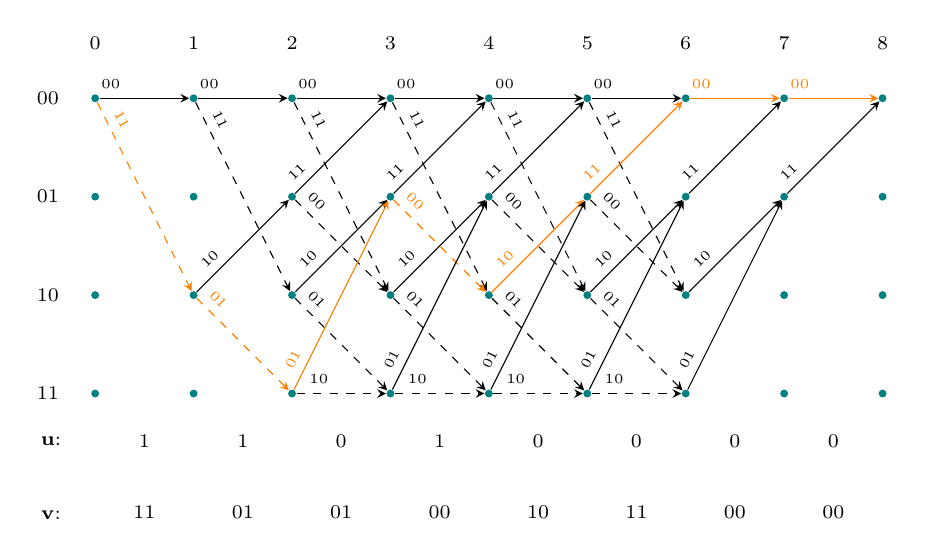
\begin{tikzpicture}[>=stealth, font=\scriptsize]
\tikzstyle{freestate} = [circle, teal, fill=teal, minimum size=1mm, inner sep=0mm]

\foreach \y in {0,...,3}
	\foreach \x in {0,...,8}
		\node[freestate] (node\y\x) at (1.25*\x,-1.25*\y) {};

\foreach \x in {0,...,8}
	\node (timelabel\x) [above of=node0\x, yshift=-3mm] {\x};
		
\node (statelabel0) [left of=node00, xshift=4mm] {00}; 
\node (statelabel1) [left of=node10, xshift=4mm] {01}; 
\node (statelabel2) [left of=node20, xshift=4mm] {10}; 
\node (statelabel3) [left of=node30, xshift=4mm] {11};

%t=0
\draw[->] (node00) -- (node01) node [sloped, above, very near start, font=\tiny] {00};
\draw[->, dashed, orange] (node00) -- (node21) node [sloped, above, very near start, font=\tiny] {11};

%t=1
\draw[->] (node01) -- (node02) node [sloped, above, very near start, font=\tiny] {00};
\draw[->, dashed] (node01) -- (node22) node [sloped, above, very near start, font=\tiny] {11};
\draw[->] (node21) -- (node12) node [sloped, above, near start, font=\tiny] {10};
\draw[->, dashed, orange] (node21) -- (node32) node [sloped, above, very near start, font=\tiny] {01};

%t=2
\draw[->] (node02) -- (node03) node [sloped, above, very near start, font=\tiny] {00};
\draw[->, dashed] (node02) -- (node23) node [sloped, above, very near start, font=\tiny] {11};
\draw[->] (node12) -- (node03) node [sloped, above, very near start, font=\tiny] {11};
\draw[->, dashed] (node12) -- (node23) node [sloped, above, very near start, font=\tiny] {00};
\draw[->] (node22) -- (node13) node [sloped, above, near start, font=\tiny] {10};
\draw[->, dashed] (node22) -- (node33) node [sloped, above, very near start, font=\tiny] {01};
\draw[->, orange] (node32) -- (node13) node [sloped, above, very near start, font=\tiny] {01};
\draw[->, dashed] (node32) -- (node33) node [sloped, above, near start, font=\tiny] {10};

%t=3
\draw[->] (node03) -- (node04) node [sloped, above, very near start, font=\tiny] {00};
\draw[->, dashed] (node03) -- (node24) node [sloped, above, very near start, font=\tiny] {11};
\draw[->] (node13) -- (node04) node [sloped, above, very near start, font=\tiny] {11};
\draw[->, dashed, orange] (node13) -- (node24) node [sloped, above, very near start, font=\tiny] {00};
\draw[->] (node23) -- (node14) node [sloped, above, near start, font=\tiny] {10};
\draw[->, dashed] (node23) -- (node34) node [sloped, above, very near start, font=\tiny] {01};
\draw[->] (node33) -- (node14) node [sloped, above, very near start, font=\tiny] {01};
\draw[->, dashed] (node33) -- (node34) node [sloped, above, near start, font=\tiny] {10};

%t=4
\draw[->] (node04) -- (node05) node [sloped, above, very near start, font=\tiny] {00};
\draw[->, dashed] (node04) -- (node25) node [sloped, above, very near start, font=\tiny] {11};
\draw[->] (node14) -- (node05) node [sloped, above, very near start, font=\tiny] {11};
\draw[->, dashed] (node14) -- (node25) node [sloped, above, very near start, font=\tiny] {00};
\draw[->,orange] (node24) -- (node15) node [sloped, above, near start, font=\tiny] {10};
\draw[->, dashed] (node24) -- (node35) node [sloped, above, very near start, font=\tiny] {01};
\draw[->] (node34) -- (node15) node [sloped, above, very near start, font=\tiny] {01};
\draw[->, dashed] (node34) -- (node35) node [sloped, above, near start, font=\tiny] {10};

%t=5
\draw[->] (node05) -- (node06) node [sloped, above, very near start, font=\tiny] {00};
\draw[->, dashed] (node05) -- (node26) node [sloped, above, very near start, font=\tiny] {11};
\draw[->,orange] (node15) -- (node06) node [sloped, above, very near start, font=\tiny] {11};
\draw[->, dashed] (node15) -- (node26) node [sloped, above, very near start, font=\tiny] {00};
\draw[->] (node25) -- (node16) node [sloped, above, near start, font=\tiny] {10};
\draw[->, dashed] (node25) -- (node36) node [sloped, above, very near start, font=\tiny] {01};
\draw[->] (node35) -- (node16) node [sloped, above, very near start, font=\tiny] {01};
\draw[->, dashed] (node35) -- (node36) node [sloped, above, near start, font=\tiny] {10};

%terminierung
%t=6
\draw[->, orange] (node06) -- (node07) node [sloped, above, very near start, font=\tiny] {00};
\draw[->] (node16) -- (node07) node [sloped, above, very near start, font=\tiny] {11};
\draw[->] (node26) -- (node17) node [sloped, above, near start, font=\tiny] {10};
\draw[->] (node36) -- (node17) node [sloped, above, very near start, font=\tiny] {01};
%t=7
\draw[->, orange] (node07) -- (node08) node [sloped, above, very near start, font=\tiny] {00};
\draw[->] (node17) -- (node08) node [sloped, above, very near start, font=\tiny] {11};

% input & output
\node (in0) at($(node30)!0.5!(node31)+(0,-.6)$) {1};
\node (in1) at($(node31)!0.5!(node32)+(0,-.6)$) {1};
\node (in2) at($(node32)!0.5!(node33)+(0,-.6)$) {0};
\node (in3) at($(node33)!0.5!(node34)+(0,-.6)$) {1};
\node (in4) at($(node34)!0.5!(node35)+(0,-.6)$) {0};
\node (in5) at($(node35)!0.5!(node36)+(0,-.6)$) {0};
\node (in6) at($(node36)!0.5!(node37)+(0,-.6)$) {0};
\node (in7) at($(node37)!0.5!(node38)+(0,-.6)$) {0};
\node (inlabel) at($(node30)+(-.56,-.6)$) {$\mathbf{u}$:};

\node (out0) [below=of in0, yshift=5mm] {11};
\node (out1) [below=of in1, yshift=5mm] {01};
\node (out2) [below=of in2, yshift=5mm] {01};
\node (out3) [below=of in3, yshift=5mm] {00};
\node (out4) [below=of in4, yshift=5mm] {10};
\node (out5) [below=of in5, yshift=5mm] {11};
\node (out6) [below=of in6, yshift=5mm] {00};
\node (out7) [below=of in7, yshift=5mm] {00};
\node (outlabel) at($(node30)+(-.56,-1.55)$) {$\mathbf{v}$:};

\end{tikzpicture}
\caption{Trellis für die terminierte Kodierung zu Beispiel~\ref{bsp:B5}}
\label{abb:trellis_terminiert}
\end{figure}
\begin{beispiel}
Gegeben sei die Nachricht $\mathbf{u}=\left( 110100\right)$ aus Beispiel~\ref{bsp:B2}. Die Kodierung der terminierten Nachricht ist in Abbildung~\ref{abb:trellis_terminiert} zu sehen und ergibt das Kodewort $\mathbf{v}=\left( 11~01~01~00~10~11~00~00\right)$.
\label{bsp:B5}
\end{beispiel}

\subsection{Punktierung}
\label{kapitel:grundlagen_punktierung}
Zur Erhöhung der Koderate $R$ eines Kodes gibt es die Möglichkeit der Punktierung. Dabei werden bestimmte Bits vor der Übertragung anhand der sogenannten \emph{Punktierungsmatrix} $P \in {\left\lbrace 0,1 \right\rbrace}^{N\times \frac{p}{N}}$ gestrichen, wobei $p$ als Periode der Punktierungsmatrix bezeichnet und $P$ spaltenweise durchlaufen wird. Das Gewicht der Matrix $w(P)$ entspricht der Anzahl nicht punktierter Kodebits je Periode, d.h. der Anzahl an Bits für die gilt $P_{ij}=1$ mit $i \in \left\lbrace 1,2,\dots ,N \right\rbrace$ und $j \in \left\lbrace 1,2,\dots ,\frac{p}{N} \right\rbrace$.~\cite[S.~218]{schonfeld2012informations}
\\
\\
Die Koderate des punktierten Kodes $R_{p}$ berechnet sich wie folgt:
\begin{equation}
R_{p}=\frac{p}{w(P)}R
\end{equation}
Vor der Dekodierung erfolgt die Depunktierung, d.h. die punktierten Kodebits werden wieder eingefügt. Bei der soft decision Dekodierung wird der Signalwert 0, also genau zwischen den eigentlichen Signalwerten +1 und -1, an den zuvor punktierten Stellen eingefügt. Bei der hard decision Dekodierung wird das Bit 0 eingefügt.

\begin{beispiel}
Gegeben sei das Kodewort $\mathbf{v}=\left( 11~01~01~00~10~11\right)$ aus Beispiel~\ref{bsp:B2} und die Punktierungsmatrix
\begin{equation*}
P=
\begin{pmatrix}
1 & 0 & 1 \\
1 & 1 & 0 \\
\end{pmatrix}.
\end{equation*}
Nach der Punktierung ergibt sich das Kodewort $\mathbf{v_{p}}=\left( 11\ast 10\ast 00\ast 01\ast\right) = \left( 11100001\right)$. Die Koderate des punktierten Kodes beträgt $R_{p}=\frac{6}{4}\cdot\frac{1}{2}=\frac{3}{4}$.
\label{bsp:B6}
\end{beispiel}

\chapter{Verwendete Technologien}
\label{kapitel:technologien}
% technologien.tex
Kapitel~\ref{kapitel:R} behandelt die Programmiersprache R und die verwendete Entwicklungsumgebung RStudio. In Kapitel~\ref{kapitel:rcpp} werden die Möglichkeiten der Einbindung von C/C++-Code, vor allem mithilfe des Pakets \texttt{Rcpp}, beschrieben. Schließlich wird in Kapitel~\ref{kapitel:rmarkdown} auf die Erstellung dynamischer Dokumente und Visualisierungen mittels \texttt{RMarkdown}, \LaTeX\ und Ti\textit{k}Z eingegangen.
\section{R, RStudio, Pakete}
\label{kapitel:R}
\begin{figure}[t]
\centering
\includegraphics[width=0.9\textwidth]{abbildungen/rstudio}
\caption{RStudio Standardansicht}
\label{abb:rstudio}
\end{figure}
% R
R ist eine, im Jahre 1992 entwickelte, schwach und dynamisch typisierte Programmiersprache, die vor allem in der Statistik für die Analyse von großen Datenmengen Anwendung findet. Ein weiteres Motiv für die Verwendung von R sind die vielseitigen Möglichkeiten, bei gleichzeitig einfacher Handhabung, große Datenmengen graphisch darzustellen. R-Code wird nicht kompiliert, sondern nur interpretiert und ist daher plattformübergreifend verwendbar. Datentypen müssen zur Übersetzungszeit nicht bekannt sein. Die Typüberprüfung findet zur Laufzeit statt. Diese Eigenschaft erschwert das Finden von Fehlern im Code erheblich.

Der Funktionsumfang der Sprache kann durch sogenannte Pakete erweitert werden. Bei der Installation von R sind die wichtigsten Pakete inkludiert. Über Repositories wie CRAN\footnote{The Comprehensive R Archive Network: \url{https://cran.r-project.org/}} oder GitHub sind über 8000 zusätzliche Pakete (Stand: Mai 2016) für die verschiedensten Anwendungsbereiche verfügbar. Diese Vielfalt an Paketen ist ein Grund für den Erfolg von R~\cite[S.~18]{wickham2015r}.
\\
Pakete werden laufend aktualisiert und verbessert. Selbst entwickelte Pakete können via CRAN für andere Entwickler veröffentlicht werden, müssen jedoch strenge Auflagen zur Aufrechterhaltung der Konsistenz bei Inhalt, Form und Dokumentation der Pakete einhalten~\cite{wickham2015r}.  

Ein wichtiges Paket, welches im Rahmen dieser Arbeit verwendet wurde, ist \texttt{roxygen2}. Mithilfe dieses Pakets wird, ähnlich zur JavaDoc für Java, durch spezielle Kommentare und Annotations überhalb der Paketfunktionen automatisch die Paketdokumentation erstellt. Die \texttt{roxygen}-Kommentare der Paketfunktionen, die für wartbaren Code ohnehin unabdingbar sind, sind für den Entwickler erheblich angenehmer, als die Paketdokumentation von Hand zu schreiben. Diese werden durch das Kommentarsymbol \mbox{\texttt{\#'}} am Zeilenbeginn eingeleitet. Zu den wichtigsten Annotations gehören jene für die Beschreibung der Parameter (\texttt{@param}) und Rückgabewerte (\texttt{@return}) sowie Beispiele zur Ausführung der Funktion (\texttt{@examples}). Weiters wird über die \texttt{@export} Annotation geregelt, welche Funktionen nach Auslieferung des Pakets von außen aufrufbar sind.~\cite{roxygen}

Ein weiteres hilfreiches Paket ist das \texttt{devtools}-Paket. Dieses Paket stellt Funktionen für die Erstellung (Build) von Paketen zur Verfügung und beschleunigt so den Build-Workflow für den Entwickler.~\cite{devtools}

% RStudio
RStudio ist eine freie open-source Entwicklungsumgebung für R. RStudio verfügt über alle notwendigen Funktionalitäten für die Softwareentwicklung mit R und bietet darüber hinaus Funktionen für eine vereinfachte Entwicklung von R-Paketen an. Abbildung~\ref{abb:rstudio} zeigt die Version 0.99.893. 
\section{C++, Rcpp}
\label{kapitel:rcpp}
Vorteile von R, wie die einfache Analyse von Datenmengen, kommen mit einem Nachteil: R ist keine schnelle Sprache. Typische Flaschenhälse sind Schleifen und rekursive Funktionen. Die Performance kann in solchen Fällen durch Auslagern von Funktionen und Algorithmen in C oder C++ erheblich verbessert werden, da der Code in diesen Sprachen kompiliert und somit optimiert werden kann, anstatt nur interpretiert zu werden.\\
R bietet drei Möglichkeiten C/C++-Code aufzurufen:
\begin{itemize}
	\itemsep-.2em % spacing between items
	\item \texttt{.C}-Schnittstelle
	\item \texttt{.Call}-Schnittstelle
	\item \texttt{Rcpp}-Paket
\end{itemize}
Die \texttt{.C}-Schnittstelle ist die einfachste Variante C-Code auszuführen, jedoch auch jene mit den größten Einschränkungen. Im C-Code sind keinerlei R-Datentypen oder R-Funktionen bekannt. Alle Argumente sowie der Rückgabewert müssen als Zeiger in der Parameterliste übergeben werden und deren Speicher muss vor dem Aufruf reserviert werden.

Bei der \texttt{.Call}-Schnittstelle handelt es sich um eine Erweiterung der \texttt{.C}-Schnittstelle. Die Implementierung ist komplexer, dafür sind R-Datentypen verfügbar und es gibt, mithilfe des \texttt{return} Statements, die Möglichkeit eines Rückgabewerts.

Sowohl bei der \texttt{.C}-Schnittstelle als auch bei der \texttt{.Call}-Schnittstelle muss der C-Code vor dem Aufruf per Hand kompiliert und in der R Session geladen werden. Das \texttt{Rcpp}-Paket ermöglicht die Verwendung von C++-Code ohne diesen Aufwand. Im C++-Code stehen R-Datentypen wie Vektoren, Matrizen oder Listen ohne komplizierte Syntax zur Verfügung. Die Funktionsaufrufe sehen, im Gegensatz zu den C-Schnittstellen, wie normale R-Funktionsaufrufe aus und machen dadurch den Code erheblich lesbarer. Weiters stehen Vektorfunktionen zur Verfügung, d.h. eine auf einen Vektor angewandte Funktion wird auf jedes Vektorelement ausgeführt und erspart somit beispielsweise eine Schleife. Bei der Entwicklung eines eigenen Pakets ist es bei der Verwendung des \texttt{Rcpp}-Pakets zusammen mit RStudio sehr einfach C++-Code zu integrieren. Durch all diese Vorteile ist das \texttt{Rcpp}-Paket die zu wählende Schnittstelle. Die genaue Verwendung des \texttt{Rcpp}-Pakets ist in \cite[S.~395~ff.]{wickham2015advanced} beschrieben.
\begin{figure}[t]
\centering
\includegraphics[width=0.9\textwidth]{abbildungen/rmarkdown}
\caption[RMarkdown Überblick]{RMarkdown Überblick, Quelle:~\cite{rmarkdown}}
\label{abb:rmarkdown}
\end{figure}
\section{RMarkdown, \LaTeX, Ti\textit{k}Z}
\label{kapitel:rmarkdown}
% R Markdown
Zur Erstellung von dynamischen Dokumenten wird das Paket \texttt{RMarkdown} verwendet. Durch die Kombination der Syntax von Markdown, R, und \LaTeX\ ergibt sich ein flexibles und einfaches Werkzeug. Die unterstützen Ausgabeformate beinhalten u.a. HTML, PDF, MS Word und Beamer (Präsentationen).

Abbildung~\ref{abb:rmarkdown} zeigt den Workflow für die Generierung eines dynamischen Dokuments mittels \texttt{RMarkdown}. Der Markdown-, R- und \LaTeX -Code wird zusammen mit dem gewünschten Ausgabeformat, wobei mehrere Angaben möglich sind, in die \texttt{RMarkdown}-Datei (Dateiendung .rmd) geschrieben. Die RMD-Datei wird dem \texttt{knitr}-Paket übergeben, welches den R-Code ausführt und eine neue Markdown-Datei (Dateiendung .md) erstellt, die den R-Code und dessen Ergebnisse beinhaltet. Die erzeugte Markdown-Datei wird von \texttt{pandoc} weiterverarbeitet, das für die Erstellung des endgültigen Dokuments im gewünschten Format zuständig ist. Bei der Verwendung von RStudio ist \texttt{pandoc} automatisch verfügbar. Den eben beschriebenen Ablauf kapselt das \texttt{RMarkdown}-Paket in einem einzigen \texttt{render}-Funktionsaufruf.

Für die Erzeugung dynamischer Grafiken wird das \LaTeX -Sprachpaket Ti\textit{k}Z verwendet. Mithilfe des Dokumenttyps Beamer in \LaTeX\ lassen sich Präsentationen erstellen. Die Grafiken und Inhalte können dadurch dynamisch ein- oder ausgeblendet, sowie farblich hervorgehoben werden. Dies ist insofern wertvoll, da Informationen, die Schritt für Schritt vervollständigt werden, es dem Benutzer leichter machen den Ablauf nachzuvollziehen. Damit Benutzer des R-Pakets dieser Arbeit die Prinzipien von Faltungskodes besser verstehen können, werden die Visualisierungen der Kodierung und Dekodierung sukzessive eingeblendet.

\chapter{Implementierung}
\label{kapitel:implementierung}
% implementierung.tex
Dieses Kapitel gibt einen Einblick in die Konzepte der Implementierung. Als Einstiegspunkt stand eine Referenzimplementierung\footnote{\url{http://vashe.org/turbo/turbo_example.c} (01.06.2016)} zur Verfügung, die den Dekodier-Algorithmus für Turbo-Kodes beinhaltet, jedoch für ein konkretes Beispiel. Dieser musste angepasst werden um für allgemeine Faltungskodes verwendbar zu sein.
\\
\\
Kapitel \ref{kapitel:implementierung_faltungskodierer} beinhaltet den Entwurf der Faltungskodierer-Datenstruktur. [TODO: Fertigstellung]
%Die Implementierung der Kodierung wird in Kapitel \ref{kapitel:implementierung_kodierung} beschrieben, die der Dekodierung in Kapitel \ref{kapitel:implementierung_dekodierung}.
%\\
%\\
%Aus Performancegründen Kodierung, Dekodierung in C++\\
%Weiters: Kodierer erzeugen, Depunktierung, Katastrophale Kodierer Prüfung (Polynom GGT mod 2)
%\\
%Parameterprüfung, Punktierung, ApplyNoise, Aufruf Visualisierung in R\\
%Referenzimplementierung
\section{Faltungskodierer}
\label{kapitel:implementierung_faltungskodierer}
Ein Faltungskodierer ist gegeben durch 
\begin{itemize}
\item $N$: Anzahl an Ausgangsbits je Eingangsbit,
\item $M$: Länge des Schieberegisters,
\item $G$: Vektor von Generatorpolynomen.
\end{itemize}
Die Angabe von $M$ ist hier redundant, jedoch Teil der Benutzereingabe zur Generierung eines Faltungskodierers, welche durch \cite{morelos2006art} inspiriert wurde.
\\
\\
Zur leichteren Implementierung der Kodierung und Dekodierung wird die Kodierer-Datenstruktur um folgende Elemente erweitert:
\begin{itemize}
\item eine \emph{Zustandsübergangsmatrix}, die angibt, in welchen Zustand der Kodierer bei einem Eingangsbit wechselt,
\item eine \emph{inverse Zustandsübergangsmatrix}, die angibt, aus welchem Zustand der Kodierer bei einem Eingangsbit kommt,
\item eine \emph{Outputmatrix}, die angibt, welche Kodebits der Kodierer bei einem Eingangsbit in einem bestimmten Zustand ausgibt,
\item ein Flag zur Markierung rekursiver systematischer Kodierer (RSC),
\item ein \emph{Terminierungsvektor} die für rekursiver systematische Kodierer angibt, ob ein Eingangsbit 0 oder 1 in einem bestimmten Zustand für die Terminierung zu verwenden ist.
\end{itemize}
Die Implementierung der Matrizen wurde aus der Referenzimplementierung übernommen, musste jedoch erweitert werden, um für allgemeine Faltungskodes verwendbar zu sein. Für alle gilt, die Anzahl an Zeilen entspricht der Anzahl an Zuständen. Der Zeilenindex entspricht dem Zustand. Die Zustandsübergangsmatrix sowie die Outputmatrix besitzen jeweils zwei Spalten. Je eine Spalte steht für ein Eingangsbit (0 oder 1), wobei der Spaltenindex dem Eingangsbit entspricht. Die inverse Zustandsübergangsmatrix benötigt eine dritte Spalte. Für viele Kodierer (v.a. nicht-rekursive) tritt der Fall ein, dass nur durch \emph{ein bestimmtes} Eingangsbit in einen bestimmten Zustand gewechselt werden kann. Sei ein Zustand bspw. nur durch das Eingangsbit 0 erreichbar, so bedeutet das, dass es für diesen Zustand mit dem Bit 0 \emph{zwei} Vorgängerzustände gibt, für ein Eingangsbit 1 jedoch keinen Vorgänger. Diese zweite Möglichkeit wird in der dritten Spalte gespeichert.
\\
\\
Der Terminierungsvektor ist für nicht-rekursive Kodierer nicht notwendig, da ein Kode eines solchen Kodierers immer mit $M$ 0-Bits terminiert wird. Bei einem rekursiven Kodierer ist es nicht trivial zu sagen mit welchem Eingangsbit in einem bestimmten Zustand terminiert wird, um den Kodierer in den Nullzustand zu bringen. Dies hängt von der Definition des Rekursionpolynoms ab. Der Terminierungsvektor wird bei der Erzeugung rekursiver Kodierer berechnet.
\\
\\
Bei der Erzeugung von Faltungskodierern ist zu prüfen ob es sich um einen katastrophalen Kodierer handelt. RSC-Kodierer sind, wie in Kapitel \ref{kapitel:grundlagen_systematische_kodierer} beschrieben, nicht zu prüfen. Zur Prüfung wird nach Theorem \ref{thm:massey} der größte gemeinsame Teiler der Generatorpolynome berechnet. Die Berechnung des größten gemeinsamen Teilers wurde mithilfe des des euklidschen Algorithmus implementiert. Sowohl der euklidsche Algorithmus als auch die dafür notwendige binäre Polynomdivision wird an eine C++ Funktion delegiert.

\section{Kodierung}
\label{kapitel:implementierung_kodierung}
Bei Faltungskodes stellt die Kodierung den bei Weitem einfacheren Teil dar. Es muss lediglich jedes Bit der zu kodierenden Nachricht zusammen mit dem aktuellen Zustand, der nach jedem Bit mithilfe der Zustandsübergangsmatrix aktualisiert wird, auf die Outputmatrix angewendet werden. Die Terminierung funktioniert analog, einzig das zu kodierende Bit muss ermittelt werden. Für RSC-Kodierer muss im Terminierungsvektor nachgeschaut werden, andernfalls ist das Bit immer 0. Abgeschlossen wird die Kodierung mit dem Abbilden der Kodebits 0 bzw. 1 auf die Signalwerte +1 bzw. -1. Algorithmus \ref{algorithmus:kodierung} zeigt den Kodierungsalgorithmus.

\begin{algorithm}[H]
\renewcommand{\algorithmicforall}{\textbf{for each}}
\caption{Faltungskodierung}
\label{algorithmus:kodierung}
\begin{algorithmic}[1]
\STATE state $=0$, code $=$ result $=$ " "
\FORALL {bit \textbf{in} message}
   \STATE output $=$ output.matrix[state][bit]
	\STATE code $=$ $concat($code, output$)$
	\STATE state $=$ state.transition.matrix$[$state$][$bit$]$
\ENDFOR
\IF{terminate code}
   \FOR {$i=0$ \TO $M-1$}
      \STATE termination.bit $=$ rsc-coder $?$ termination.vector$[$state$]$ : $0$
      \STATE output $=$ output.matrix$[$state$][$termination.bit$]$
	   \STATE code $=$ $concat($code, output$)$
	   \STATE state $=$ state.transition.matrix$[$state$][$termination.bit$]$
   \ENDFOR
\ENDIF
\FORALL {bit \textbf{in} code}
   \STATE signal $=1-2$bit
   \STATE result $=$ $concat($result,signal$)$
\ENDFOR
\RETURN result
\end{algorithmic}
\end{algorithm}

\section{Dekodierung}
\label{kapitel:implementierung_dekodierung}
Die Dekodierung stellt den wesentlich komplexeren Teil der Faltungskodes dar. 

\begin{algorithm}[H]
\renewcommand{\algorithmicforall}{\textbf{for each}}
\caption{Faltungsdekodierung}
\label{algorithmus:dekodierung}
\begin{algorithmic}[1]
\STATE $NUM_STATES=2^{M}$
\FOR {$t=1$ \TO $length($message$)$}
   \FOR {$s=0$ \TO $NUM_STATES-1$}
   	\STATE $m_{1}=$ metric[t-1][prev.state1] + $\delta_{1}$
   	\STATE $m_{2}=$ metric[t-1][prev.state2] + $\delta_{2}$
      \STATE metric[t][s] = $min(m_{1},m_{2})$
      \STATE survivor.bit $=$ $xyz(0,1,min(min(m_{1},m_{2}))$
	\ENDFOR
\ENDFOR
\RETURN result
\end{algorithmic}
\end{algorithm}

\section{Rauschen}
\label{kapitel:implementierung_noise}
Um auch zeigen zu können, dass die Dekodierung auch tatsächlich für verrauschte Signale funktioniert, benötigt es eine Funktion, die die Übertragung einer Nachricht über einen verrauschten Kanal simuliert, d.h. das Signal mit Rauschen überlagert. Zum Signal soll ein additives weißes gaußsches Rauschen (AWGR oder AWGN\footnote{additive white Gaussian noise}) addiert werden um dieses zu verfälschen. [apply noise quelle] stellt eine alternative Implementierung zur eingebauten AWGN-Funktion in Matlab vor. Die Implementierung wurde übernommen bzw. nach R übersetzt. Durch die Möglichkeit das Signal-Rausch-Verhältnis über einen Parameter zu steuern, können verschiedene Übertragungskanäle simuliert und Nachrichten somit verschieden stark verrauscht werden. Der Benutzer kann dadurch herausfinden, ab wann eine Nachricht zu viel Rauschen enthält, um sie korrekt dekodieren zu können. Weiters kann nach mehrfacher Ausführung auf Fehlermuster geschlossen werden, mit denen die Dekodierung gut bzw. schlecht umgehen kann. Durch Versuche mit anderen Kanalkodierungs-Methoden können Vergleiche mit diesen angestellt werden. Die genannten Punkte helfen dem Benutzer sein Verständnis für Faltungskodes noch besser zu stärken.

\section{Punktierung}
\label{kapitel:implementierung_punktierung}
Punktierung leicht, jedoch Depunktierung vor der Dekodierung nicht trivial.

%\section{Visualisierung}
%\label{kapitel:implementierung_visualisierung}

\startlist[Funktionen]{lot}
\chapter{R-Paket Schnittstelle}
\label{kapitel:interface}
% R Paket Schnittstelle für Faltungskodierung
\definecolor{lightblue}{RGB}{150,180,255}

\section{Kanalkodierung}
\label{chapter:interface_kanalkodierung}
\begin{longtable}{|p{\textwidth}|}
\hline
\rowcolor{lightblue}
ApplyNoise\\
\hline
\\
\texttt{ApplyNoise(msg, SNR.db, binary)}\\
\\
Verrauscht ein Signals basierend auf das AWGN (additive white gaussian noise) Modell. Das ist das Standardmodell für die Simulation eines Übertragungskanals.\\
\\
\textbf{Argumente:}\\
\texttt{msg} - Nachricht die verrauscht wird.\\
\texttt{SNR.db} - Signal/Rausch-Verhältnis des Übertragungskanals. Standard: 3.0\\
\texttt{binary} - Blockkode-Parameter. Nicht zu verwenden! Standard: FALSE\\
\\
\textbf{Rückgabewert:}\\
Verrauschtes Signal.\\
\\
\hline
\caption{ApplyNoise - Funktionserklärung}
\end{longtable}
\stoplist[Funktionen]{lot}

\chapter{Visualisierung}
\label{kapitel:visualisierung}
% visualisierung.tex
LIMITS!\\\\
%Da das R-Paket für Studenten zu Lernzwecken verwendet werden soll
Um das Verständnis für Faltungskodes beim Benutzer dieses R-Pakets zu stärken, stehen Visualisierungen der Kodierung und Dekodierung zur Verfügung.
\\
Wird der \texttt{visualize} Parameter bei der Ausführung einer Funktion zur Kodierung oder Dekodierung auf TRUE~\texttt{TRUE} gesetzt, wird ein R Markdown Skript ausgeführt. Dieses generiert eine Beamer Präsentation mit Informationen und Visualisierungen zur Kodierung bzw. Dekodierung.
\\\\
\textcolor{lightgray}{\ref{chapter:visualisierung}.1 Kodierung}\\
% allg. Informationen
Bei der Kodierung befinden sich auf den ersten Folien allgemeine Informationen zum verwendeten Faltungskodierer wie die Kode-Rate, Generatorpolynome, Zustandsübergangstabelle etc. 
% Kodierung
Daraufhin folgt die Kodierungsvisualisierung. Diese zeigt zunächst die zu kodierende Nachricht (Input), das Zustandsübergangsdiagramm sowie eine noch nicht befüllte Kodierungstabelle. Um für einen noch besseren Lerneffekt zu sorgen wird Schritt für Schritt mittels Overlays ein Bit des Inputs, der aktuelle Zustand, Folgezustand sowie der resultierende Output in eine neue Zeile der Kodierungstabelle geschrieben. Der aktuelle Zustand sowie der entsprechende Übergang werden im Diagramm farblich hervorgehoben. Die kodierte Nachricht wächst mit jedem Schritt bis schlussendlich die gesamte Nachricht kodiert wurde.
% Kode zu Signal
Da die Kodierungsfunktion nicht die Bitwerte des Kodeworts zurückliefert sondern die Signalwerte (für eine Übertragung über einen Kanal) wird auf einer weiteren Folie dargestellt, wie die Kodebits in Signalwerte überführt werden.\\
% Punktierung
Wird eine Punktierungsmatrix bei der Kodierung mitgegeben, wird eine zusätzliche Folie am Ende hinzugefügt. Auf dieser wird die Punktierung des Signals, d.h. das Entfernen von Signalwerten (definiert durch die Punktierungsmatrix) dargestellt. Dabei wird neben dem originalen Signal und der Punktierungsmatrix das punktierte Signal dargestellt, wobei zunächst die punktierten Signalwerte, d.h. die entfernten Werte, durch Asterisk-Symbole (\textasteriskcentered) ersetzt werden. Diese Darstellung dient als visueller Zwischenschritt für das danach folgende tatsächlich punktierte Signal, bei dem die punktierten Werte fehlen, was auch dem Rückgabewert der Funktion entspricht.
\\\\
\textcolor{lightgray}{\ref{chapter:visualisierung}.2 Dekodierung}\\
% allg. Informationen
Bei der Dekodierung befinden sich ebenfalls, wie bei der Kodierung, allgemeine Informationen des Faltungskodierers auf den ersten Folien.
% Signal zu Kode
Als Input erhält die Dekodierung das Kodewort als Signalwerte, die möglicherweise durch Anwendung der \texttt{ApplyNoise} Funktion verfälscht worden sind. Die soft decision Dekodierung verwendet zur Dekodierung zwar kontinuierliche Signalwerte, da aber sowohl die hard decision Dekodierung Bitwerde zur Dekodierung verwendet und Trellis-Diagramme mit Bitwerten beschriftet werden, wird auf einer Folie die Überführung der Signalwerte zu Bits dargestellt. Dieser transformierte Input wird auch als Input für die Visualisierung des Viterbi-Algorithmus verwendet.
% Viterbi-Algorithmus
Anschließend folgt die Visualisierung des Viterbi-Algorithmus mithilfe des Trellis-Diagramms. Zunächst werden, zur besseren Übersicht bei großen Diagrammen, jene Pfade entfernt, für die es eine bessere Alternative gibt, d.h. die eine größere Metrik bei hard decision Dekodierung bzw. eine kleinere Metrik bei soft decision Dekodierung als ihre Alternative haben. Danach erfolgt Schritt für Schritt mittels Backtracking die Rekonstruktion der Nachricht. Der gewählte Pfad beim Backtracking wird farblich hervorgehoben. Die übrigen Pfade werden ausgegraut. Am Ende befindet sich unter dem Trellis-Diagramm die farblich hervorgehobene dekodierte Nachricht.
% Punktierung
Wird eine Punktierungsmatrix bei der Dekodierung mitgegeben, wird eine zusätzliche Folie nach den Kodiererinformationen hinzugefügt. Auf dieser wird die Depunktierung des Signals, d.h. das Einfügen des Signalwerts 0 (definiert durch die Punktierungsmatrix), dargestellt. Die eingefügten 0-Werte sind zur leichteren visuellen Erkennung farblich hervorgehoben.
\\\\
\textcolor{lightgray}{\ref{chapter:visualisierung}.3 Simulation}\\
Weiters können Berichte der Simulation generiert werden, die die resultierenden Daten u.a. in einem Diagramm darstellen.

\chapter{Beispiele}
\label{kapitel:beispiele}
% beispiele.tex
In diesem Kapitel werden Beispiele zur Verwendung der R-Paket Funktionen der Faltungskodierung veranschaulicht und erklärt. Kapitel~\ref{kapitel:beispiele_kodierer} führt Variablen ein, die über die weiteren Beispiele hinweg verwendet werden. Die Kapitel~\ref{kapitel:beispiele_kodieren_ohneP} bzw. \ref{kapitel:beispiele_kodieren_mitP} beinhalten die Kodierung und Dekodierung ohne bzw. mit Punktierung. Schließlich werden in Kapitel~\ref{kapitel:beispiele_simulation} Beispiele für die Ausführung von Simulationen vorgestellt. 

\section{Erzeugen von Kodierer und Punktierungsmatrix}
\label{kapitel:beispiele_kodierer}
Vor den Beispielen der Kodierung und Dekodierung werden Hilfsvariablen definiert, die für die folgenden Beispiele verwendet werden. Variablen wie der Faltungskodierer oder die Punktierungsmatrix müssen jedoch nicht unbedingt bei der Kodierung oder Dekodierung mitgegeben werden. Fehlt bei den Parametern der Kodierer, wird der Standard-Faltungskodierer aus Beispiel~\ref{bsp:B1} verwendet. Gibt man keine Punktierungsmatrix mit, so wird das Signal auch nicht punktiert. Die meisten weiteren Parameter (Terminierung, Visualisierung etc.) besitzen auch Standardwerte, die verwendet werden, falls vom Benutzer keine Werte bestimmt werden.
\begin{lstlisting}[caption=Erzeugung von Kodierer und Punktierungsmatrix, label={listing:kodierer_erzeugen}, float=!th]
input <- c(1,0,1,1,0)
 
nasa.encoder <- ConvGenerateEncoder(2, 6, c(171,133))

p.matrix <- ConvGetPunctuationMatrix(c(1,0,1,1,0,1), nasa.encoder)
p.matrix
     [,1] [,2] [,3]
[1,]    1    1    0
[2,]    0    1    1
\end{lstlisting}
Listing~\ref{listing:kodierer_erzeugen} zeigt die Erzeugung der Variablen für die weitern Beispiele. Zunächst wird eine Quellnachricht \texttt{input} erzeugt, gefolgt von der Definition des NASA-Standardkodierers~\cite[S. 90]{morelos2006art}. Zuletzt wird eine Punktierungsmatrix aus dem mitgegebenen Punktierungsvektor und dem verwendeten Kodierer generiert. Der Kodierer ist notwendig, da die Anzahl der Zeilen der Punktierungsmatrix gleich der Anzahl der Kodiererausgänge $N$ ist (siehe Kapitel~\ref{kapitel:grundlagen_punktierung}).

\section{Kodieren und Dekodieren ohne Punktierung}
\label{kapitel:beispiele_kodieren_ohneP}
Im folgenden Beispiel wird eine Nachricht kodiert, verfälscht und sowohl mithilfe der soft decision Dekodierung als auch mithilfe der hard decision Dekodierung dekodiert.
\begin{lstlisting}[caption=Kodierung und Dekodierung ohne Punktierung, label={listing:kodierung_u_dekodierung_ohneP}, float=!tbh]
encoded <- ConvEncode(input, nasa.encoder)
encoded
[1] -1 -1 -1  1  1  1 -1  1  1 -1  1 -1  1  1  1 -1 -1  1 -1 -1  1  1
 
encoded.noisy <- ApplyNoise(encoded, SNR.db = 0.2)
round(encoded.noisy, 2)
[1] -0.83 -0.75 -0.36  1.31  1.05  0.16  0.37 -0.12  1.55 -0.92  3.48 -1.31  0.22  2.49  1.07 -1.19 -1.02  2.00 -1.40 -0.78  1.12  0.50

decoded.soft <- ConvDecodeSoft(encoded.noisy, nasa.encoder)
decoded.soft
$output.soft
[1] -6.67485  6.67485 -6.67485 -6.67485  6.67485

$output.hard
[1] 1 0 1 1 0

decoded.hard <- ConvDecodeHard(encoded.noisy, nasa.encoder)
decoded.hard
[1] 1 0 1 1 0
\end{lstlisting}
Listing~\ref{listing:kodierung_u_dekodierung_ohneP} beinhaltet den Code zur Kodierung und Dekodierung ohne Punktierung. Für die Kodierung der Nachricht wird diese einfach zusammen mit dem Kodierer der Kodierungsfunktion \texttt{ConvEncode} übergeben. Als Resultat erhält man das Kodewort mit den Signalpegeln +1 bzw. -1. Anschließend wird dieses mit der \texttt{ApplyNoise}-Funktion und einem Signal-Rausch-Verhältnis von 0,2dB verrauscht und der \texttt{encoded.noisy} Variable zugewiesen. Die Ausgabe dient dem Vergleich des unverfälschten und des verrauschten Kodeworts. Die Werte werden aus Platzgründen auf zwei Nachkommastellen gerundet. Schließlich erfolgt die soft decision und die hard decision Dekodierung. Der Rückgabewert der soft decision Dekodierung ist eine Liste welche sowohl die Soft-Werte als auch die Hard-Werte beinhaltet. Die hard decision Dekodierung gibt nur einen Vektor mit den dekodierten Bits 0 bzw. 1 zurück. Das Beispiel zeigt die Fähigkeit der Faltungskodierung, stark verrauschte Signale korrekt dekodieren zu können.

\section{Kodieren und Dekodieren mit Punktierung}
\label{kapitel:beispiele_kodieren_mitP}
Das kodierte Signal kann vor der Übertragung zur Verbesserung der Koderate punktiert werden. Die Punktierung streicht anhand der Punktierungsmatrix Bits aus dem Kodewort, wie in Kapitel~\ref{kapitel:grundlagen_punktierung} beschrieben. Im folgenden Beispiel wird eine Nachricht kodiert und punktiert bevor sie dekodiert wird.
\begin{lstlisting}[caption=Kodierung und Dekodierung mit Punktierung, label={listing:kodierung_u_dekodierung_mitP}, float=!th]
encoded.punctured <- ConvEncode(input, nasa.encoder, punctuation.matrix = p.matrix)
encoded.punctured
$original
[1] -1 -1 -1  1  1  1 -1  1  1 -1  1 -1  1  1  1 -1 -1  1 -1 -1  1  1

$punctured
[1] -1 -1  1  1 -1  1 -1 -1  1  1 -1  1 -1  1  1

decoded.soft <- ConvDecodeSoft(encoded.punctured$punctured, nasa.encoder, punctuation.matrix = p.matrix)
decoded.soft
$output.soft
[1] -6  5 -5 -5  5

$output.hard
[1] 1 0 1 1 0

decoded.hard <- ConvDecodeHard(encoded.punctured$punctured, nasa.encoder, punctuation.matrix = p.matrix)
decoded.hard
[1] 1 0 1 1 0
\end{lstlisting}
Die Kodierung und Dekodierung mit Punktierung ist in Listing~\ref{listing:kodierung_u_dekodierung_mitP} zu sehen. Die Punktierung erfolgt durch das Mitgeben der Punktierungsmatrix bei der Kodierung. Das Ergebnis der Kodierung ist eine Liste mit dem originalen (nicht punktierten) Signal und dem punktierten Signal. Bei der weiteren Verwendung der Variable ist zu beachten, dass nicht die gesamte Liste zu verwenden ist, sondern nur das originale oder punktierte Listenelement. Dies ist beim Aufruf der Dekodierung zu sehen. Die Dekodierung benötigt auch die Punktierungsmatrix für das Auffüllen der punktierten Stellen im Kodewort. Als Ergebnis erhält man, wie bei der Dekodierung ohne Punktierung, eine Liste der Soft-Werte und Hard-Werte bei der soft decision Dekodierung bzw. einen Vektor der dekodierten Nachricht bei der hard decision Dekodierung.

\section{Simulation}
\label{kapitel:beispiele_simulation}
Die folgenden Kapitel demonstrieren die verschiedenen Möglichkeiten Simulationen durchzuführen. Kapitel~\ref{kapitel:beispiele_simulation_faltungskodierung} beinhaltet ein Beispiel für eine Simulation der Faltungskodierung. Eine Simulation der drei Verfahren der Kanalkodierung des R-Pakets (Blockkodes, Faltungskodes und Turbo-Kodes) wird in Kapitel~\ref{kapitel:beispiele_simulation_kanalkodierung} präsentiert. Kapitel~\ref{kapitel:beispiele_simulation_vergleich} beinhaltet eine Beispielanwendung der Hilfsfunktion zur Darstellung verschiedener Simulationsergebnisse.

\subsection{Faltungskodierung}
\label{kapitel:beispiele_simulation_faltungskodierung}
Das folgende Beispiel zeigt die Ausführung einer Simulation der Faltungskodierung. Die Parameter der Funktion wie der verwendete Kodierer, die Nachrichtenlänge, die zu testenden Signal-Rausch-Verhältnisse, die Anzahl an Wiederholungen je Signal-Rausch-Verhältnis sowie die Punktierungsmatrix können bestimmt werden, sind jedoch auch mit Standardwerten hinterlegt.
\begin{lstlisting}[caption=Simulation der Faltungskodierung, label={listing:ConvSimulation}, float=!th]
> df1 <- ConvSimulation(nasa.encoder, msg.length = 2000, min.db = 0.01, max.db = 0.1, db.interval = 0.01, iterations.per.db = 100)

df1
     db      ber
1  0.01 0.151810
2  0.02 0.140220
3  0.03 0.150020
4  0.04 0.143695
5  0.05 0.142150
6  0.06 0.142900
7  0.07 0.138555
8  0.08 0.137155
9  0.09 0.141615
10 0.10 0.137050
\end{lstlisting}
Listing~\ref{listing:ConvSimulation} zeigt die Simulation mithilfe der \texttt{ConvSimulation}-Funktion. Auf eine Punktierung wird in diesem Beispiel verzichtet. Die Länge der getesteten Nachrichten beträgt 2000 Bits. Diese werden bei einem Signal-Rausch-Verhältnis zwischen 0,01dB und 0,1dB verrauscht und im Anschluss dekodiert. Es wird der Mittelwert der Bitfehlerraten über 100 Wiederholungen je Signal-Rausch-Verhältnis gebildet. Der Rückgabewert der Simulation ist ein Dataframe, welches die Bitfehlerrate (\texttt{ber}) je Signal-Rausch-Verhältnis (\texttt{db}) beinhaltet. Für eine Visualisierung kann der Visualisierungs-Parameter der Funktion gesetzt werden (\texttt{visualize = TRUE}) um einen Simulationsbericht als PDF-Datei generieren zu lassen. Eine weitere Möglichkeit bietet die in Kapitel~\ref{kapitel:beispiele_simulation_vergleich} präsentierte Hilfsfunktion.

\subsection{Kanalkodierung}
\label{kapitel:beispiele_simulation_kanalkodierung}
Für einen Vergleich aller drei Verfahren der Kanalkodierung, die dieses R-Paket umfasst, kann die Funktion \texttt{ChannelcodingSimulation} verwendet werden. Diese Funktion ist eine Wrapper-Funktion, die jede Simulationsfunktion der verschiedenen Kanalkodierungen mit den gleichen Parametern aufruft und die resultierenden Bitfehlerraten in ein Dataframe schreibt und zurückgibt. Das Beispiel in Listing~\ref{listing:ChannelcodingSimulation} führt eine Simulation für eine Nachrichtenlänge von 2000 Bits aus. Die getesteten Signal-Rausch-Verhältnisse liegen zwischen 0,01dB und 0,1dB. Je Signal-Rausch-Verhältnis werden 100 Wiederholungen zur Ermittlung der Bitfehlerrate durchgeführt. Die Dekodierung der Turbo-Kodes erfolgt mit 3 Iterationen. Für eine Visualisierung der Daten kann der Visualisierungs-Parameter der Funktion gesetzt werden (\texttt{visualize = TRUE}) um einen Simulationsbericht als PDF-Datei generieren zu lassen.
\begin{lstlisting}[caption=Kanalkodierungs-Simulation, label={listing:ChannelcodingSimulation}, float=!th]
ChannelcodingSimulation(msg.length = 2000, min.db = 0.01, max.db = 0.1, db.interval = 0.01, iterations.per.db = 100, turbo.decode.iterations = 3)

     db block.ber conv.ber turbo.ber
1  0.01  0.197045 0.088875  0.051680
2  0.02  0.197095 0.088670  0.051570
3  0.03  0.195555 0.090415  0.051935
4  0.04  0.196410 0.089065  0.052815
5  0.05  0.193475 0.089780  0.052700
6  0.06  0.194410 0.090370  0.050620
7  0.07  0.195250 0.089125  0.049625
8  0.08  0.194870 0.086845  0.050740
9  0.09  0.192465 0.089515  0.049495
10 0.10  0.193470 0.084220  0.048935
\end{lstlisting}

\subsection{Vergleich von Simulationen}
\label{kapitel:beispiele_simulation_vergleich}
Das folgende Beispiel zeigt die Ausführung der \texttt{PlotSimulationData}-Funktion. Mithilfe dieser Funktion lassen sich die mit den Simulationsfunktionen erzeugten Dataframes in einem Plot darstellen, was den Vergleich erheblich vereinfacht. In Listing~\ref{listing:PlotSimulationData} wird zunächst ein zweites Dataframe erstellt, welches mit dem in Listing~\ref{listing:ConvSimulation} erstellten Dataframe visualisiert werden soll. Als Vergleich wird ein katastrophaler Faltungskodierer (siehe Kapitel~\ref{kapitel:grundlagen_katastrophale_kodierer}) erzeugt, mit dem die Simulation zur Erzeugung von \texttt{df2} ausgeführt wird. Abbildung~\ref{abb:PlotSimulationData} zeigt den erzeugten Plot.
\begin{lstlisting}[caption=Vergleich mehrerer Simulationsdaten, label={listing:PlotSimulationData}, float=!th]
catastrophic.encoder <- ConvGenerateEncoder(2,2,c(6,5))
df2 <- ConvSimulation(catastrophic.encoder, msg.length = 2000, min.db = 0.01, max.db = 0.1, db.interval = 0.01, iterations.per.db = 100)

df2
     db      ber
1  0.01 0.492040
2  0.02 0.502815
3  0.03 0.490140
4  0.04 0.497805
5  0.05 0.499780
6  0.06 0.489430
7  0.07 0.496505
8  0.08 0.504305
9  0.09 0.493600
10 0.10 0.490645

PlotSimulationData(df1,df2)
\end{lstlisting}
\begin{figure}[!ht]
	\centering
	\includegraphics[width=\ScaleIfNeeded]{abbildungen/Rplot_PlotSimulationData}
	\caption{Plot zweier Simulations-Dataframes}
	\label{abb:PlotSimulationData}
\end{figure}

\chapter{Zusammenfassung und Ausblick}
\label{kapitel:fazit}
% fazit.tex
Diese Arbeit beinhaltet die Implementierung von Faltungskodes, einem Verfahren zur Kanalkodierung, innerhalb eines R-Pakets. Außerdem stehen Funktionen für Blockkodes und Turbo-Kodes zur Verfügung, welche aus anderen Bachelorarbeiten stammen. Dadurch ergibt sich ein kompaktes und vielseitig verwendbares R-Paket für die Kanalkodierung. Das entwickelte R-Paket besitzt einen beachtlichen Funktionsumfang, u.a. stehen Funktionen zur Kodierung, Dekodierung und Simulation verschiedener Kanalkodierungen zur Verfügung.
\\
\\
In erster Linie wurde das Paket zu Lehrzwecken für zukünftige Studierende entwickelt. Diese sollen durch die Verwendung des Pakets die Prinzipien der Faltungskodierung bzw. Kanalkodierung verstehen können. Dabei helfen dynamisch generierte Visualisierungen, welche die Kodierung, Dekodierung und Simulation veranschaulichen.
\\
\\
Erweiterungspotenzial besteht vor allem im Bereich der Visualisierung:
\begin{itemize}
\item Schaltbild des Faltungskodierers\\Die Darstellung der Zustandsdiagramme der Kodierer ist nur bei einer Schieberegisterlänge von maximal drei möglich. Durch die Darstellung mittels des Kodierer-Schaltbilds könnten auch Kodierer mit längeren Schieberegistern dargestellt werden, ohne unübersichtlich zu werden.
\item Berechnung der Metriken der Dekodierung\\Eine Darstellung der Herleitung bzw. Erklärung zur Berechnung der Metriken gäbe den Werten, aus der Perspektive des Benutzers, mehr Bedeutung.
\item Berechnung der Soft-Werte der soft decision Dekodierung\\Eine Darstellung, wie sich die Soft-Werte der soft decision Dekodierung errechnen, würde dem Benutzer helfen die resultierenden Soft-Werte interpretieren zu können.
\end{itemize}
Der Funktionsumfang des Pakets könnte weiters durch die Implementierung des BCJR-Algorithmus erweitert werden. Mit dem BCJR-Algorithmus existiert eine etwas komplexere Alternative zum Viterbi-Algorithmus zur Dekodierung von Faltungskodes. Anstelle der Suche nach dem wahrscheinlichsten Pfad im Trellis wird ein Pfad gesucht, sodass die Fehlerwahrscheinlichkeit der einzelnen Bits minimal ist \cite[S.~233~ff.]{schonfeld2012informations}.

\cleardoublepage%

%\listofabbreviations
%\clearpage

\listoffigures
\clearpage

%\printlist[tables]{lot}{}{\renewcommand\addvspace[1]{}\chapter*{Tabellenverzeichnis}}
%\clearpage

\lstlistoflistings
\clearpage

\listofalgorithms
\clearpage

\printlist[Funktionen]{lot}{}{\renewcommand\addvspace[1]{}\chapter*{Funktionsverzeichnis}}
\clearpage

\defbibheading{myheading}[Literatur]{\chapter*{#1}}
\pagestyle{plain}
\printbibliography[heading=myheading]
\end{document}
